\chapter{End of chapter exercise solutions}
\label{eoceSolutions}



%_______________
\eocesolch{Introduction to data}



%_______________
\begin{multicols}{2}

%% 9.1 CASE STUDY: PREVENTING PEANUT ALLERGIES
	
% 1

\eocesol{(a)~Treatment: $10/43 = 0.23 \rightarrow 23\%$. \\
	Control: $2/46 = 0.04 \rightarrow 4\%$. \\
(b)~At first glance, it appears patients in the treatment group seem more 
likely to experience pain reduction from the acupuncture treatment. There is a 19\% difference between the pain reduction rates in the two 
groups, with the treatment group experiencing the higher pain reduction rate.}

% 2 

\eocesol{(a)~Treatment: $66/85 = 0.78 \rightarrow 78\%$ of patients in the treatment group experienced a significant improvement in symptoms. \\
	Control: $66/81 = 0.80 \rightarrow 80\%$ of patients in the control group experienced a significant improvement in symptoms. \\
	(b)~The control group's symptomatic treatments appear to be more effective than the treatment group's amoxicillin treatment because the control group has a higher percentage of patients who reported significant improvement in symptoms than the treatment group (80\% vs. 78\%). \\
	(c)~Answers may vary but should be sensible. Possible answer: Because the observed 2\% difference is rather small, the observed difference may well be simply due to chance.}


%% 9.2 DATA BASICS


% 3

\eocesol{(a)~143,196 eligible study subjects born in Southern California between 1989 
	and 1993. \\
	(b)~Measurements of carbon monoxide, nitrogen dioxide, ozone, and particulate 
	matter less than 10$\mu g/m^3$ (PM$_{10}$) collected at air-quality-monitoring 
	stations as well as length of gestation. Continuous numerical variables.  \\
	(c)~"Is there an association between air pollution 
	exposure and incidence of preterm births?"}

% 4

\eocesol{(a)~600 asthma patients, ages 18-69.  \\
	(b)~Scores on quality of life, activity, asthma symptoms, and medication reduction on a scale from 0 to 10. Ordinal categorical variables. \\
	(c)~"Is there evidence that the Buteyko method reduces asthma and improves quality of life?"}

% 5

\eocesol{(a)~The control tests are the ones in which hummingbirds are presented with either sucrose or water. The treatment tests are the ones in which hummingbirds are presented with test stimuli (aspartame, erythritol). \\
	(b)~Length of time a hummingbird drank from each of the two containers in a given trial. Numerical variable. \\
	(c)~"Does the T1R1-T1R3 taste receptor in hummingbirds play a role in detecting sweetness?"}

% 6

\eocesol{(a)~Control: the group of 16 female birds that received no treatment. Treatment: the group of 16 female birds that were given supplementary diets. \\
	(b)~"Does egg coloration indicate the health of female collared flycatchers?" \\
	(c)~Darkness of blue color in female birds' eggs. Continuous numerical variable.}

% 7

\eocesol{(a)~Each row represents a participant. \\
	(b)~1,691 participants. \\
	(c)~Sex: nominal categorical variable. Age: discrete numerical variable. Marital status: nominal categorical variable. Gross income: ordinal categorical variable. Smoking status: nominal categorical variable. Amount of smoking during weekends: discrete numerical variable. Amount of smoking during weekdays: discrete numerical variable.}

% 8

\eocesol{(a)~Each row represents a participant. \\
	(b)~The response variable is colon cancer stage. The explanatory variables are the abundance levels of the five bacterial species. \\
	(c)~Colon cancer stage: ordinal categorical variable. Abundance levels of bacterial species: continuous numerical variable.  }

% 9 

\eocesol{(a)~The population of interest consists of babies born in Southern California. The sample consists of the 143,196 babies born between 1989 and 1993 in Southern California. \\
	(b)~Assuming that the sample is representative of the population of interest, the results of the study can be generalized to the population. The findings cannot be used to establish causal relationships because the study was an observational study, not an experiment.}

% 10

\eocesol{(a)~The population of interest consists of asthma patients who rely on medication for asthma treatment. The sample consists of the 600 asthma patients ages 18-69 who participated in the study. \\
	(b)~The sample may not be representative of the population because study participants were recruited, an example of a convenience sample. Thus, the results of the study may not be generalizable to the population. The findings can be used to establish causal relationships because the study is an experiment conducted with control, randomization, and a reasonably large sample size.}


% 11

\eocesol{(a)~The population of interest consists of healthy young adults. The sample consists of the 437 healthy young adult volunteers from the University of Virginia. \\
	(b)~The sample may not be representative of the population because study participants were volunteers, an example of a convenience sample. Additionally, participants were all from the University of Virginia community; it is possible that there may be a systematic difference between these young adults and those in the wider population. Thus, the results may not be generalizable to the population. Even so, many studies rely on this kind of convenience sampling. \\
  (c)~The findings can be used to establish causal relationships because the study is an experiment conducted with a control, randomization, and a reasonably large sample size.}

%% 9.3 DATA COLLECTION PRINCIPLES

% 12

\eocesol{(a)~Experiment. The researchers directly intervened and assigned treatments, manipulating the explanatory variable to examine changes in the response variable. \\
	(b)~The explanatory variable is the dose of Vitamin C taken at the onset of a cold. The response variables are cold duration and severity. \\
	(c)~Yes, there may be underlying differences between participants who choose to take the pill and participants who choose not to take the pill. The researcher's analysis may introduce confounding if it is only based on the participants who chose to take the pill.}

% 13

\eocesol{(a)~Experiment.  \\
	(b)~The treatment group consists of the individuals assigned to exercise twice a week. The control group consists of of the individuals instructed not the exercise. \\
	(c)~Yes. The blocking variable is age. \\
	(d)~The results of the study can be used to establish a causal relationship because the study is an experiment. Since the only systematic difference between the groups was the difference in the explanatory variable, it is reasonable to attribute the observed changes in the response variable to differences in the explanatory variable. The conclusions can be generalized to the larger population since the sample is representative of the population. \\
	(e)~Answers may vary. Possible answer: A more complex study design may be required in order to account for differences in participants' usual exercise habits. In the current design, individuals in the treatment group are simply instructed to exercise twice a week; for some, this could be an increase in exercise, and others, this could be a decrease. To address this issue, the treatment group participants could be instructed to exercise once a week more than usual, while the control group participants are instructed to maintain their current exercise regime. In the analysis, participants would need to be compared according to their initial exercise regimes.}

% 14

\eocesol{(a)~Experiment. \\
	(b)~The experimental group consists of the chicks that received vitamin supplements. The control group consists of the chicks that did not receive vitamin supplements. \\
	(c)~Randomization ensures that there are not systematic differences between the control and treatment groups. Even if chicks may vary in ways that affect body mass and corticosterone levels, random allocation essentially evens out such differences, on average, between the two groups. This is essential for a causal interpretation of the results to be valid.}


% 15

\eocesol{(a)~Observational study. \\
	(b)~Answers may vary. One possible confounding variable is the wealth of a country. A wealthy country's citizens tend to have a higher life expectancy due to a higher quality of life, and the country tends to have a higher percentage of internet users because there is enough money for the required infrastructure and citizens can afford computers. Wealth of a country is associated with both estimated life expectancy and percentage of internet users. Omitting the confounder from the analysis distorts the relationship between the two variables, such that there may seem to be a direct relationship when there is not.}

% 16

\eocesol{(a)~Observational study. \\
	(b)~No, observational studies can only establish correlation. \\
	(c)~Answers may vary. One possible confounding variable is final exam period. Final exam period may increase both student stress (students may study more and sleep less) and muscle cramps (students may be less active because they are studying).}

% 17 

\eocesol{(a)~Simple random sampling is reasonable if 500 students is a large enough sample size relative to the total student population of the university. \\
	(b)~Since student habits may vary by field of study, stratifying by field of study would be a reasonable decision. \\
	(c)~Students in the same class year may have more similar habits. Since clusters should be diverse with respect to the outcome of interest, this would not be a good approach.}

% 18

\eocesol{(a)~Non-responders may have a different response to this question, e.g. 
parents who returned the surveys likely don't have difficulty spending time 
with their children. \\
(b)~It is unlikely that the women who were reached at the same address 3 years 
later are a random sample. These missing responders are probably renters 
(as opposed to homeowners) which means that they might be in a lower socio-economic class than the respondents. \\
(c)~This is an observational study, not an experiment, so it is not advisable to draw conclusions about causal relationships. The relationship may be in the other direction; i.e., that these people go running precisely because they do not have joint problems. Additionally, the data are not even sufficient to provide evidence of an association between running and joint problems because data have only been collected from individuals who go running regularly. Instead, a sample of individuals should be collected that includes both people who do and do not regularly go running; the number of individuals in each group with joint problems can then be compared for evidence of an association.}

% 19

\eocesol{(a)~Effective. The random sample will likely be representative of the city. \\
	(b)~Effective. This method ensures that each neighborhood is represented in the sample. A feature of this sample is that each neighborhood will be represented by an equal number of households; this is not, however, necessarily reflective of neighborhood sizes in the city. In a simple random sample, households from smaller neighborhoods are less likely to be chosen, and vice versa for households from larger neighborhoods; this leads to a sample that is strictly representative of the population. \\
	(c)~Not effective. It seems likely that neighborhoods are more variable than the households within a single neighborhood; thus, it is inefficient to sample all the households in a selected neighborhood. \\
	(d)~Effective. This addresses the issue with the sampling strategy in (c). \\
	(e)~Not effective. The sample would not be representative of the city since households closer to the city council offices may share characteristics that households farther from the city do not have. This sampling method would result in a biased sample.}

% 20 

\eocesol{(a)~No. The study is an observational study, so only conclusions about correlation can be drawn. However, it is important to note that an experiment would not be ethical here. \\
	(b)~No, because it implies a causal relationship between sleep disorders and bullying. In this case, we can at most conclude that there is a correlation between symptoms of sleep disorders and bullying in school children.}

% 21 

\eocesol{The lead author's statements are not accurate because he or she drew conclusions about causation (that increased alcohol sales taxes lower rates of sexually transmitted infections) from an observational study. In addition, although the study observed that there was a decline in gonorrhea rate, the lead author generalized the observation to all sexually transmitted infections.}


%% 9.4 NUMERICAL DATA

% 22
\eocesol{(a)~The two distributions have the same median since they have the same middle number when ordered from least to greatest. Distribution 2 has a higher IQR because its first and third quartiles are farther apart than in Distribution 2. \\
	(b)~Distribution 2 has a higher median since it has a higher middle number when ordered from least to greatest. Distribution 2 has a higher IQR because its first and third quartiles are farther apart than in Distribution 1. \\
	(c)~Distribution 2 has a higher median since all values in this distribution are higher than in Distribution 1. The two distributions have the same IQR since the distance between the first and third quartiles in each distribution is the same. \\
	(d)~Distribution 2 has a higher median since most values in this distribution are higher than those in Distribution 1. Distribution 2 has a higher IQR because its first and third quartiles are farther apart than those of Distribution 1.}

% 23

\eocesol{(a)~Distribution~2 has a higher mean since $20 > 13$, and a higher standard deviation 
since 20 is further from the rest of the data than 13. \\
(b)~Distribution~1 has a higher mean since $-20 > -40$, and Distribution~2 has a 
higher standard deviation since -40 is farther away from the rest of the data than -20. \\
(c)~Distribution~2 has a higher mean since all values in this distribution are higher 
than those in Distribution~1, but both distribution have the same standard deviation 
since they are equally variable around their respective means. \\
(d)~Both distributions have the same mean since they are both centered at 300, but 
Distribution~2 has a higher standard deviation since the observations are farther from 
the mean than in Distribution~1.}

% 24

\eocesol{(a)~Symmetric, centered at 60. Boxplot 2.
	(b)~Symmetric, centered at 50. Boxplot 3.
	(c)~Right skew, centered at 1. Boxplot 1.}

% 25

\eocesol{(a)~The distribution is bimodal, with peaks between 15-20 and 25-30. Values range from 0 to 65.  \\
(b)~The median AQI is about 30. \\
(c)~I would expect the mean to be higher than the median, since there is some right skewing.}

% 26 

\eocesol{(a)~Symmetric. There are no outliers; the boxplot does not show points outside the range of the whiskers. \\
	(b)~ Answers may vary. The histogram is more informative because it provides a more detailed picture of how the data are distributed, while the boxplot does not provide information about the overall shape of the distribution. Alternatively, the boxplot more clearly shows the median and interquartile range. \\
	(c)~Answers may vary. Various factors could influence the number of elderly people in a given state who choose to live in nursing homes. In states that are more sparsely populated, more residents might choose to stay in nursing homes because of the difficulties associated with living in rural areas, such as absence of easily accessible medical care. In wealthier states, however, people are less likely to live in nursing homes because of their ability to afford the costs of staying home (e.g. in-home nursing care); Social Security, Medicare, and Medicaid pay quite a lot of nursing home costs.}

% 27

\eocesol{(a)~The distribution of the scores show right skew. The scores range from 0 to about 18, with the majority of scores under 10. \\
	(b)~Since the distribution is skewed, the robust measures of center and spread, median and IQR, provide a better summary of the data.}

% 28

\eocesol{No, the midrange is sensitive to outliers and extreme skew since it is calculated using the two most extreme values in the distribution. If the extreme values in the distribution change, then the midrange will change, even if the rest of the distribution did not change.}

%% 9.5 CATEGORICAL DATA

% 29

\eocesol{(a)~Conservatives: 372/910 = 0.41 $\rightarrow$ 41\% \\
	(b)~In favor of the citizenship option: 278/910 = 0.31 $\rightarrow$ 31\% \\
	(c)~Conservative and in favor of the citizenship option: 57/910 = 0.06 $\rightarrow$ 6\% \\
	(d)~In favor of the citizenship option among conservatives: 57/372 = 0.15 $\rightarrow$ 15\% 
	In favor of the citizenship option among moderates: 120/363 = 0.33 $\rightarrow$ 33\%
	In favor of the citizenship option among liberals: 101/175 = 0.58 $\rightarrow$ 58\%}

% 30

\eocesol{(a)~These data are categorical. They can be summarized numerically in either a frequency table or relative frequency table, and summarized graphically in a bar plot of either counts or proportions. \\
	(b)~The results of these studies cannot be generalized to the larger population. Individuals taking the survey represent a specific subset of the population that are conscious about dental health, since they are at the dentist's office for an appointment. Additionally, there may be response bias; even though the surveys are anonymous, it is likely that respondents will feel some pressure to give a "correct" answer in such a setting, and claim to floss more often than they actually do.}

%% 9.6 RELATIONSHIPS BETWEEN TWO VARIABLES

% 31

\eocesol{(a)~Yes, there seems to be a positive association between lifespan and length of gestation. Generally, as gestation increases, so does life span. \\
	(b)~Positive association. Reversal of the plot axes does not change the nature of an association.}

% 32

\eocesol{(a)~Plot 1, linear. Plot 3, nonlinear.
	(b)~Plot 4, linear.
	(c)~Plot 2.}

% 33

\eocesol{(a)~75\% of the countries have an adolescent fertility rate less than or equal to 75.73 births per 1,000 adolescents. \\
	(b)~It is likely that the observations are missing due to the Iraq War and general instability in the region during this time period. It is unlikely that the five-number summary would have been affected very much, even if the values were extreme; the median and IQR are robust estimates, and the dataset is relatively large, with data from 188 other countries. \\
	(c)~The median and IQR decreases each year, with Q1 and Q3 also decreasing.}

% 34 

\eocesol{(a)~51/215 = 0.24 $\rightarrow$ 24\% of the participants were both smokers and had aortic stenosis. The other three numbers of the joint distribution are: 54/215 = 0.25 $\rightarrow$ 25\% (percent of participants who were smokers and did not have aortic stenosis); 43/215 = 0.20 $\rightarrow$ 20\% (percent of participants who were non-smokers and had aortic stenosis); and 67/215 = 0.31 $\rightarrow$ 31\% (percent of participants who were non-smokers and did not have aortic stenosis). \\
	(b)~Among the 105 smokers, 51 have aortic stenosis. Thus, 51/105 of the smokers have aortic stenosis. Among the 110 non-smokers, 43 have aortic stenosis. Thus, 43/110 of the non-smokers have aortic stenosis. \\
	(c)~The relative risk of aortic stenosis, comparing smokers to non-smokers, is $\frac{51/105}{43/110} = 1.24$. The risk of a smoker developing aortic stenosis is 1.24 times that of a non-smoker. Since the relative risk is greater than 1, there does seem to be evidence that smoking is associated with an increased probability of stenosis. The relative risk is also greater than 1.2, indicating that a smoker's probability of stenosis is alarmingly higher than that of a non-smoker.}

% 35

\eocesol{(a)~4,371/8,474 = 0.56 $\rightarrow$ 56\% \\
	(b)~110/190 = 0.58 $\rightarrow$ 58\% \\
	(c)~27/633 = 0.04 $\rightarrow$ 4\% \\
	(d)~53/3,110 = 0.02 $\rightarrow$ 2\% \\
	(e)~Relative risk: $\frac{27/633}{53/3,110} = 2.50$. Yes, since the relative risk is greater than 1. A relative risk of 2.50 indicates that individuals with high trait anger are 2.5 times more likely to experience a CHD event than individuals with low trait anger. \\
	(f)~Side-by-side boxplots, since blood cholesterol level is a numerical variable and anger group is categorical.}

%_______________
\end{multicols}


\textC{\newpage}



%_______________
\eocesolch{Probability}

%% 2.1 DEFINING PROBABILITY

%_______________
\begin{multicols}{2}

% 1

\eocesol{(a)~False. These are independent trials. \\
(b)~False. There are red face cards. \\
(c)~True. A card cannot be both a face card and an ace.}

% 2

\eocesol{(a)~0. It is impossible to roll a pair of dice and get a sum of one. The smallest possible sum is 2 (1 and 1). \\
	(b)~$\frac{4}{36}$. There are 4 possible pairs sum to 5 (1 and 4; 2 and 3; 3 and 2; 4 and 1) and a total of 36 possible pairs (6 x 6), giving a probability of $\frac{\text{number of pairs that sum to 5}}{\text{total number of pairs}}$ = $\frac{4}{36}$. \\
	(c)~$\frac{1}{36}$. There is one possible pair that sums to 12 (6 and 6) and a total of 36 possible pairs (6 x 6), giving a probability of $\frac{\text{number of pairs that sum to 12}}{\text{total number of pairs}}$ = $\frac{1}{36}$.}

% 3

\eocesol{(a)~$\frac{1}{4}$. \\
	Solution 1: A colorblind male has genotype $X^{-}Y$. He must have inherited $X^{-}$ from his mother (probability of $\frac{1}{2}$) and $Y$ from his father (probability of $\frac{1}{2}$). Since these are two independent events, the probability of both occuring is $(\frac{1}{2}) (\frac{1}{2}) = \frac{1}{4}$. \\
	Solution 2: Determine the possibilities using a Punnett square. There are 4 equally likely possibilities, one of which is a colorblind male. Thus, the probability is $\frac{1}{4}$. 
	
	\begin{center}
		\begin{tabular}{ |c|c|c| } 
			\hline
			& $X^{+}$ & $Y$ \\ 
			\hline
			$X^{+}$ & $X^{+}X^{+}$ & $X^{+}Y$ \\ 
			\hline
			$X^{-}$ & $X^{+}X^{-}$ & $X^{-}Y$ \\ 
			\hline
		\end{tabular}
	\end{center}
	(b)~True. An offspring of this couple cannot be both female and colorblind.}

% 4

\eocesol{(a)~No. Someone can have diabetes and hypertension. \\
	(b)\\
	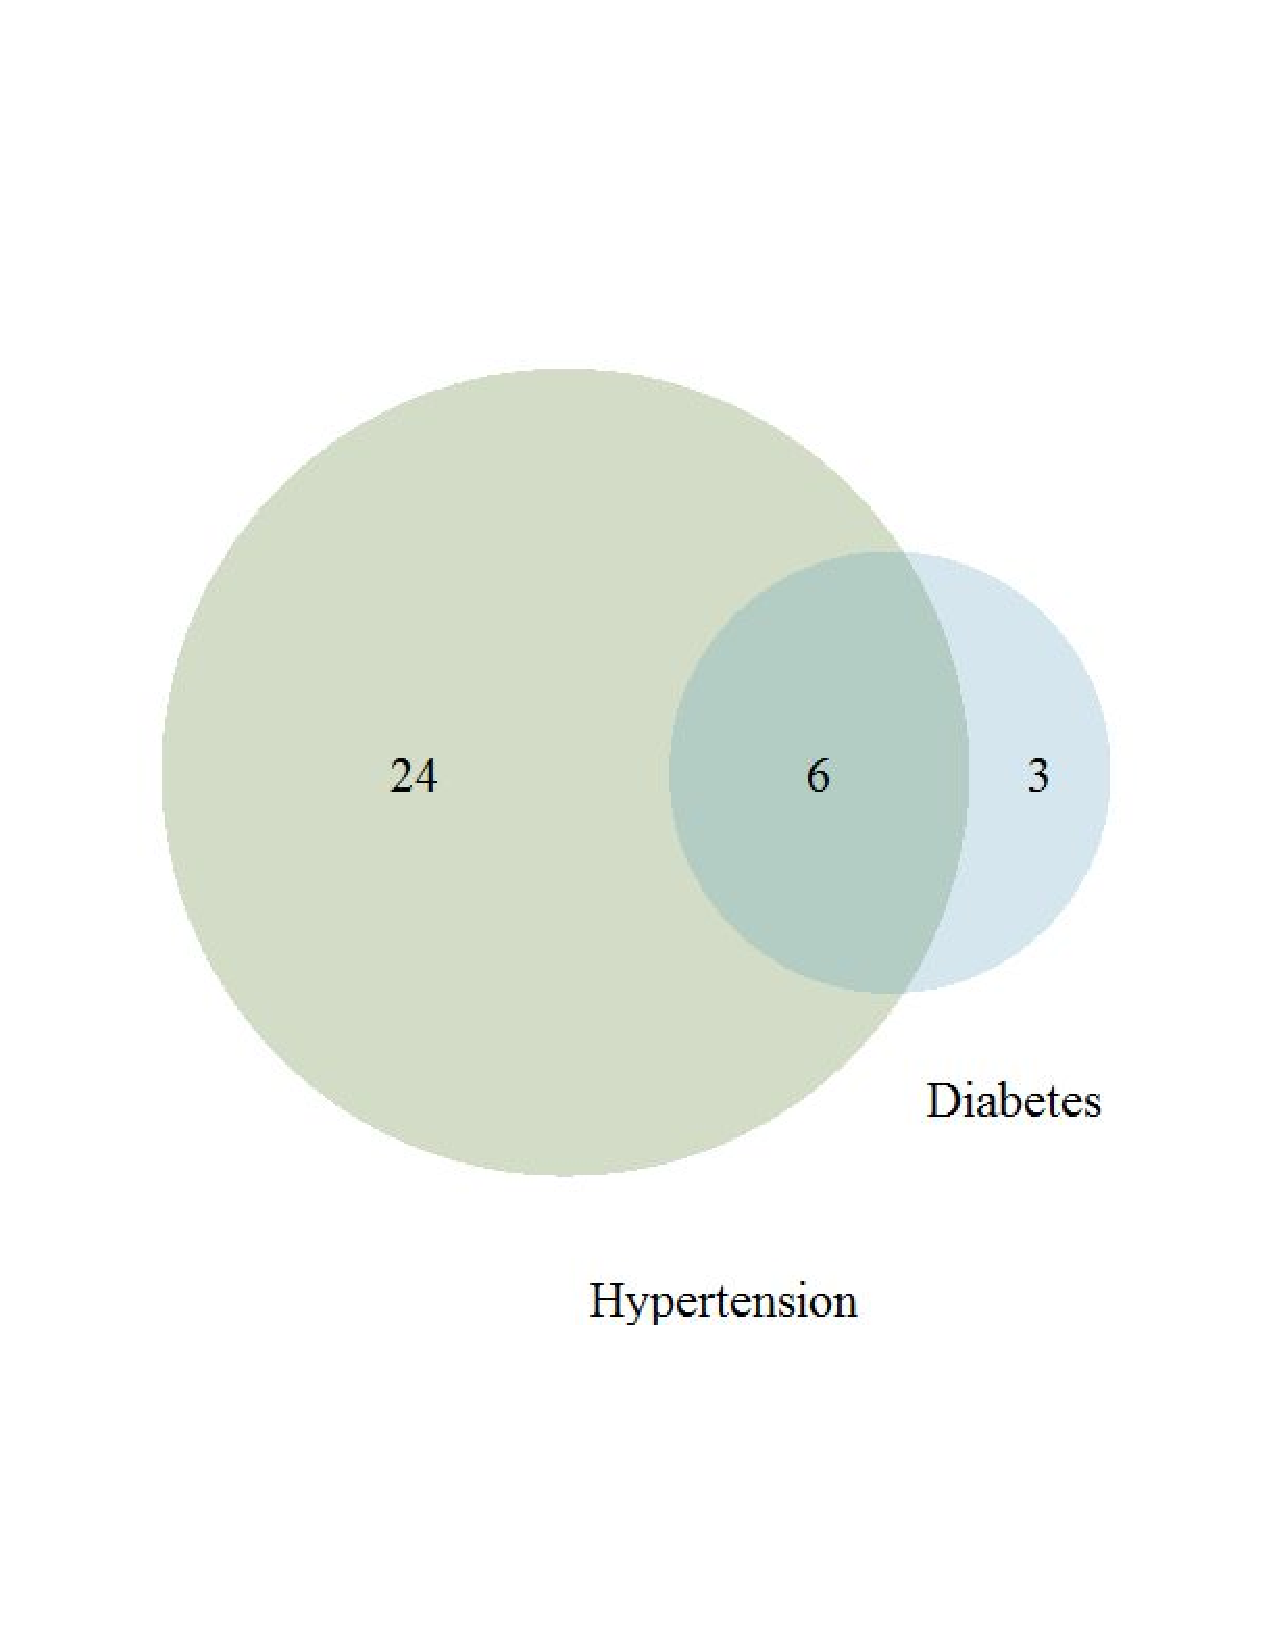
\includegraphics[width=40mm]{ch_probability_oi_biostat/figures/eoce/diabetes_hypertension/diabetes_hypertension.pdf} \\
	(c)~0.33. $P(\text{$A$ or $B$}) = P(A) + P(B) - P(\text{$A$ and $B$}) = 0.09 + 0.30 - 0.06 = 0.33$. \\
	(d)~67\%. $P(\text{$A^{C}$ and $B^{C}$}) = 1 - P(\text{$A$ or $B$}) = 1 - 0.33 = 0.67 = 67\%$. \\
	(e)~No. If diabetes (A) and hypertension (B) were independent, $P(\text{$A$ and $B$}) = P(A)P(B)$. Since $0.06 \neq (0.09)(0.30)$, i.e. $P(\text{$A$ and $B$}) \neq P(A)P(B)$, the events are not independent.}

% 5

\eocesol{(a)~No. Someone can live below the poverty line and speak a foreign language at home. \\
	(b)
	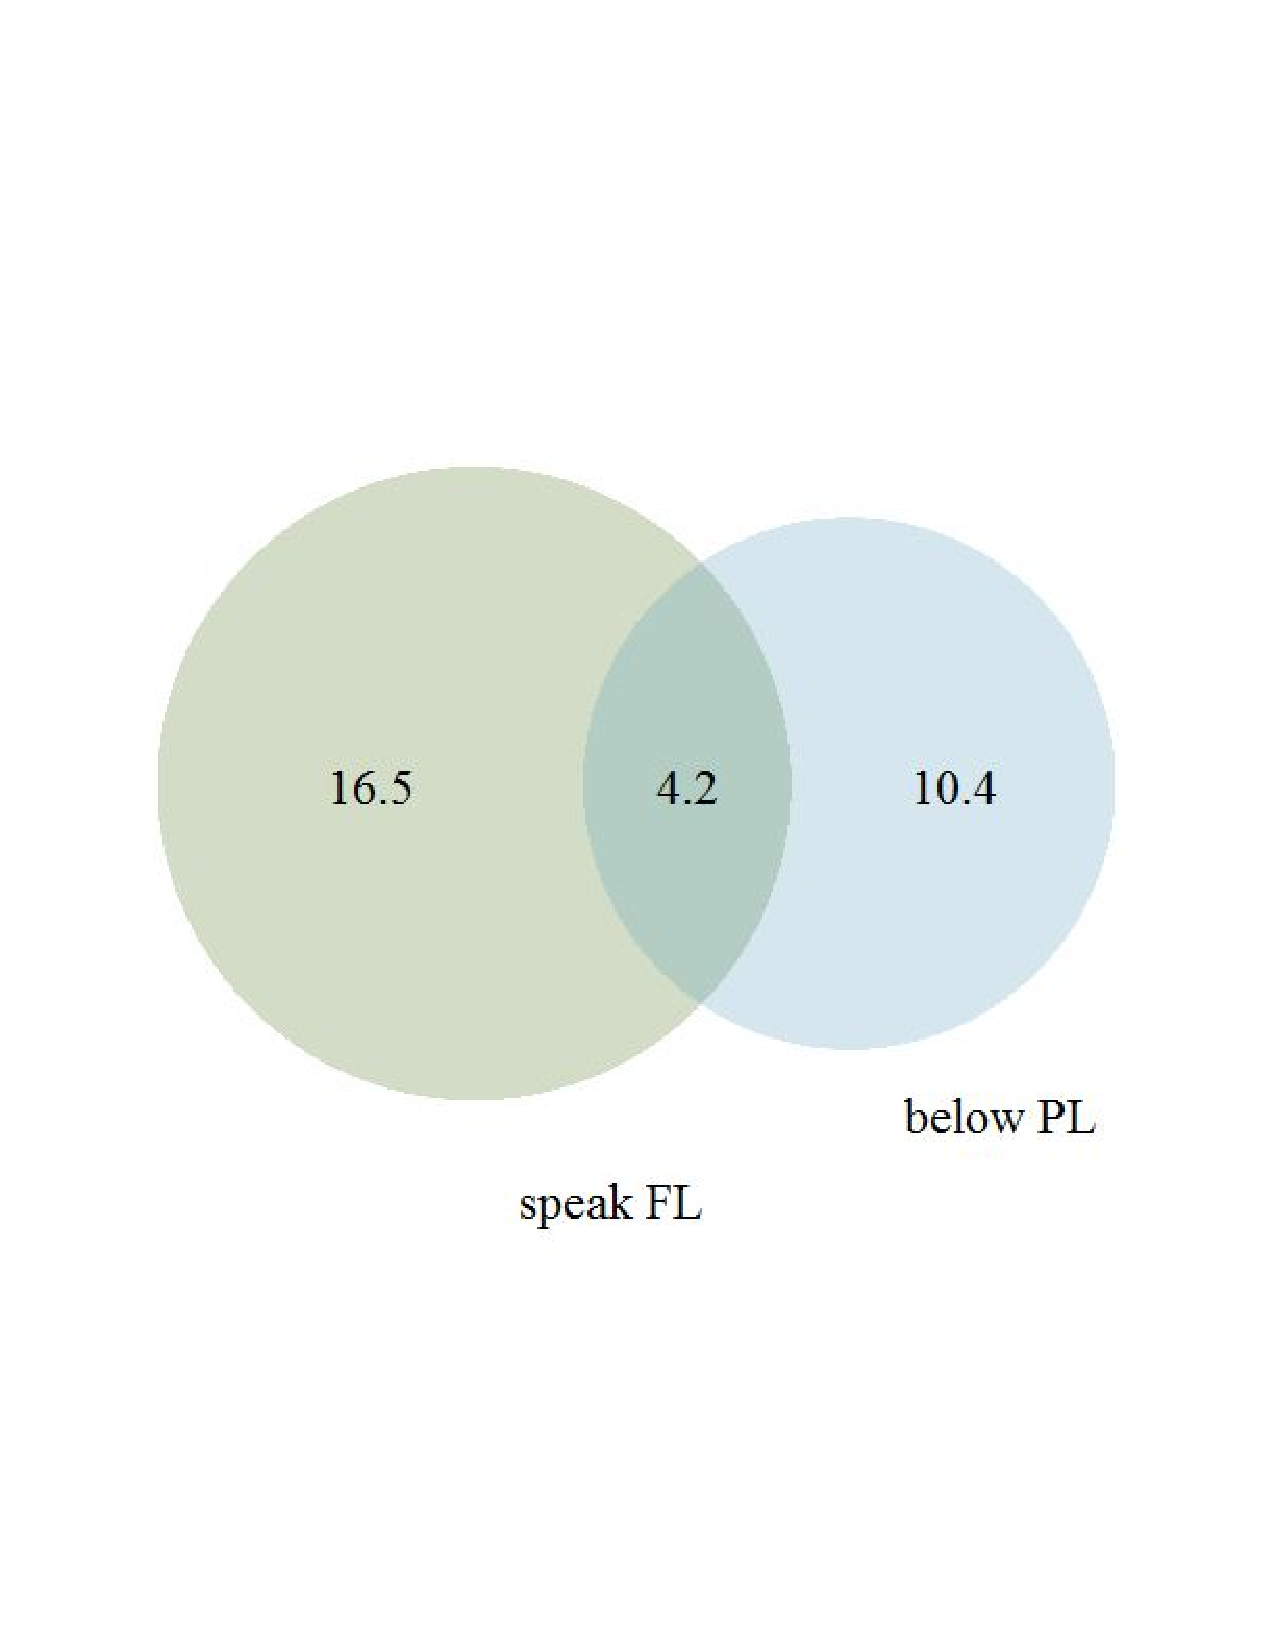
\includegraphics[width=40mm]{ch_probability_oi_biostat/figures/eoce/poverty_language/poverty_language.pdf} \\
	(c)~10.4\%. \\
	Solution 1: The "10.4\%" portion of the Venn diagram represents Americans who live below the poverty line and do not speak a foreign language at home (i.e. only speak English at home).
	Solution 2: Let $A$ = \{living below the poverty line\} and $B$ = \{speaking a foreign language at home\}. Given $P(A) = 0.146$, $P(B) = 0.207$, and $P(A \textrm{ and }B) = 0.042$, calculate $P(A \textrm { and } B^C)$. $P(A \textrm{ and }B^C) = P(A)P(B^C | A) = P(A)(1 - P(B|A)) = P(A)(1 - \frac{P(A \textrm{ and } B)}{P(A)}) = (0.146)(1 - \frac{0.042}{0.146}) = 0.104 \rightarrow 10.4\%$  \\
	(d)~31.1\%. $P(A \textrm{ or } B) = P(A) + P(B) - P(A \text{ and } B) = 0.146 + 0.207 - 0.042 = 0.311 \rightarrow 31.1\%$. \\
	(e)~68.9\%. The group of Americans who live above the poverty line and only speak English at home is represented in the Venn diagram by the space in the rectangle but outside either of the two circles. $P(A^{C} \text{ and } B^{C}) = 1- P(A \text{ or } B) = 1- 0.311 = 0.689 = 68.9\%$. \\
	(f)~No. If $A$ and $B$ were independent events, then $P(\text{$A$ and $B$}) = P(A)P(B)$. Since $0.042 \neq (0.146)(0.207)$, i.e. $P(\text{$A$ and $B$}) \neq P(A)P(B)$, the events are not independent.
	}
	
\textC{\end{multicols}
%\end{multicols}
\newpage
\begin{multicols}{2}}

% 6 

\eocesol{(a)~0.25. Let $H$ represent the event of being a high school graduate and $F$ represent the event of being a woman. $P(H) = P(H \textrm{ and } W) + P(H \textrm{ and } W^C) = P(H|W)P(W) + P(H|W^C)P(W^C) = (0.20)(0.50) + (0.30)(0.50) = 0.25$. \\
	(b)~0.91.$(A^C) = P(A^C \textrm{ and } W) + P(A^C \textrm{ and } W^C) = (1-0.09) + (1-0.09) = 0.91$. \\
	(c)~0.25. Let $X$ represent the event of having at least a Bachelor's degree, where $B$ represents the event of attaining at most a Bachelor's degree and $G$ the event of attaining at most a graduate or professional degree.  $P(X|W^C) = P(B|W^C) + P(G|W^C) = 0.16 + 0.09 = 0.25$. \\
	(d)~0.26. $P(X|W) = P(B|W) + P(G|W) = 0.17 + 0.09 = 0.26$. \\
	(e)~0.065. Let $X_W$ be the event that a woman has at least a Bachelor's degree, and $X_M$ be the event that a man has at least a Bachelor's degree. Assuming that the education levels of the husband and wife are independent, $P(X_W \textrm{ and } X_M) = P(X_W) \times P(X_M) = (0.25)(0.26) = 0.065$. This assumption is probably not reasonable, because people tend to marry someone with a comparable level of education.
}

% 7 

\eocesol{(a)~0.32. Let $D_0$, $D_1$, $D_2$, $D_3$ represent the events of missing 0, 1, 2, and 3 or more days of school per year. $P(D_0) = 1 - P(D_0^C) = 1 - (P(D_1) + P(D_2) + P(D_3)) = 1- (0.25 + 0.15 + 0.28) = 0.32$. \\
	(b)~0.57. The probability of missing at most 1 day is equal to missing either 0 days or 1 day: $P(D_0) + P(D_1) = 0.32 + 0.25 = 0.57$.\\
	(c)~0.68. The probability of missing at least 1 day is equal to missing either 1, 2, or 3 or more days: $P(D_1) + P(D_2) + P(D_3) = 0.25 + 0.15 + 0.28.$. This can also be thought of as the complement of missing 0 days: $1 - P(D_0) = 1 - 0.32 = 0.68$.\\
	(d)~0.10. Assuming that the school attendance of one child is independent of that of the other child, $P(D_0) \times P(D_0) = (0.32)(0.32) = 0.10$. This assumption is probably not reasonable because the attendance of children from the same household is typically correlated. For example, the two children may have a parent that takes them to school at the same time. \\
	(e)~0.46. Assuming that the school attendance of one child is independent of that of the other child, $(0.68)(0.68) = 0.46$. This assumption is probably not reasonable because the attendance of children from the same household is typically correlated. For example, if one child becomes ill and cannot go to school, it is likely that the other child will also be ill and cannot go to school.}

% 8 

\eocesol{(a)~Let $C$ represent the event that one urgent care center sees 300-449 patients in a week. Assuming that the number of patient visits are independent between urgent care centers in a given county for a given week, the probability that three random urgent care centers see 300-449 patients in a week is $[P(C)]^3 = (0.288)^3 = 0.024$. This assumption is not reasonable because a county is a small area with relatively few urgent care centers; if one urgent care center takes in more patients than usual during a given week, so might other urgent care centers in the same county (e.g., this could occur during flu season). \\
	(b)~$2.32 \times 10^{-7}$. Let $D$ represent the event that one urgent care center sees 450 or more patients in a week. Assuming independence, the probability that 10 urgent care centers throughout a state all see 450 or more patients in a week is $[P(D)]^{10} = (0.217)^{10} = 2.32 \times 10^{-7}$. This assumption is reasonable because a state is a large area that contains many urgent care centers; the number of patients one urgent care center takes in is likely independent of the number of patients another urgent care center in the state takes in. \\
	(c)~No, it is not possible, because it is not reasonable to assume that the patient visits for a given week are independent of those for the following week.}


% 9

\eocesol{(a)~$459/20,000 = 0.023$. \\
	(b)~Let $A$ be the event of having excellent health and $B$ be the event of not having health coverage. $P(A \textrm{ or } B) = P(A) + P(B) - P(A \textrm{ and } B) = \frac{4,657}{20,000} + \frac{2,524}{20,000} - \frac{459}{20,000} = \frac{6,722}{20,000} = 0.336$. }




\textC{\end{multicols}
\newpage
\begin{multicols}{2}}

%% 2.1 CONDITIONAL PROBABILITY

% 10 (oi biostat)

\eocesol{(a)~0.25. Each parent can pass on either an A allele or a B allele with probability 0.5. For a child to have Group A blood, they must inherit an A allele from both parents. Alleles are inherited independently, thus, the probability of a child of this couple having Group A blood is $(0.50) \times (0.50) = 0.25$. \\
	(b)~0.141. The probability that one child has Type O blood is $(0.50) \times (0.50) = 0.25$, since the child must inherit the $i$ allele from both parents. The probability that a child does not have Type O blood is $1 - 0.25 =0.75$ (the complement). Each child inheriting alleles is an independent event. The probability that their first child has Type O blood and the next two do not is: $(0.25) \times (0.75) \times (0.75) = 0.141$. \\
	(c)~1/3. The event that one child has Type O blood and two do not can happen three distinct ways: either the first, second, or third child is the one child with Type O blood. Neither child is more or less likely to have Type O blood, so the conditional probability that it is the first child given the stated condition equals $1/3$ by symmetry. This can also be approached algebraically; let $A$ be the event that the first child has Type O blood and $B$ be the event that one child has Type O blood and two do not.
	\[P(A|B) = \dfrac{P(A \cap B)}{P(B)} = \dfrac{(0.25)(0.75)(0.75)}{(3)(0.25)(0.75)(0.75)} = \dfrac{1}{3} \] }

% 11

\eocesol{(a)~$0.60 + 0.20 - 0.18 = 0.62$ \\
	(b)~$0.18/0.20 = 0.90$ \\
	(c)~$0.11/0.33 = 0.33$ \\
	(d)~No, because the answers to parts (c) and (d) are not equal. If global warming belief were independent of political party, then among liberal Democrats and conservative Republicans, there would be equal proportions of people who believe the earth is warming. \\
	(e)~$0.06/0.34 = 0.18$ }

% 12

\eocesol{(a)~No. Someone can be in excellent health and have health coverage. \\
	(b)~0.2329. \\
	(c)~$0.2099/0.8738 = 0.2402$. \\
	(d)~$0.0230/0.1262 = 0.1823$. \\
	(e)~No. let $A$ represent the event of being in excellent health and $B$ represent the event of having health coverage. Under independence, $P(A \textrm{ and }B ) = P(A)P(B)$. Since $0.2099 \neq (0.2329)(0.8738)$, the events are not independent.}

% 13
\eocesol{(a)~$375,264/436,968 = 0.859$ \\
	(b)~$229,246/255,980 = 0.896$ \\
	(c)~0.896. This is equivalent to (b). \\
	(d)~$146,018/180,988 = 0.807$ \\
	(e)~$4,719/7,394 = 0.638$ \\
	(f)~No, because the answers to (c) and (d) are not equal. If gender and seat belt usage were independent, then among males and females, there would be the same proportion of people who always wear seat belts.}

% 14

\eocesol{(a)~$\frac{114 + 108 - 78}{204} = \frac{144}{204} = 0.706$. \\
	(b)~$\frac{78}{114} = 0.684$. \\
	(c)~$19/54 = 0.352$. $11/36 = 0.306$. \\
	(d)~No, because the answers to (b) and (c) are not equal. If the male respondents' eye colors were independent of their partners' eye colors, then among male respondents with blue eyes, brown eyes, and green eyes, there would be the same proportion who have partners with blue eyes.}

% 15 (oi, edited)

\eocesol{(a)~0.6049. \\ $P(D|T^{+}) = 
	\frac{P(T^{+}|D)P(D)}{P(T^{+}|D)P(D) + P(T^{+}|D^C)P(D^C)} = \\ \frac{(0.99)(0.03)}{(0.99)(0.03) + (1-0.98)(1-0.03)} = 0.6049$. \\
	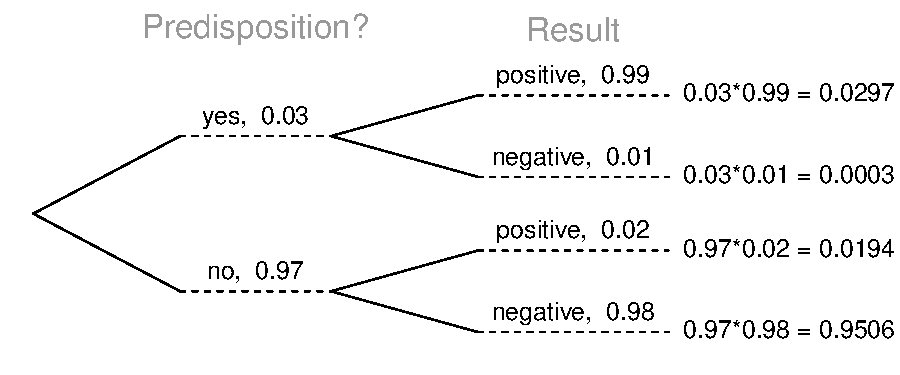
\includegraphics[width=60mm]{ch_probability_oi_biostat/figures/eoce/tree_thrombosis/tree_thrombosis.pdf}
	(b)~0.9994. \\ $P(D^C|T^{-}) = 
	\frac{P(T^{-}|D^C)P(D^C)}{P(T^{-}|D^C)P(D^C) + P(T^{-}|D)P(D)} = \\ \frac{(0.98)(1-0.03)}{(0.98)(1-0.03) + (1-0.99)(0.03)} = 0.9994$. \\}

% 16 (oi, edited)
\eocesol{The PPV is 0.8248. The NPV is 0.9728. \\ $P(D|T^{+}) = 
	\frac{P(T^{+}|D)P(D)}{P(T^{+}|D)P(D) + P(T^{+}|D^C)P(D^C)} = \\ \frac{(0.997)(0.0259)}{(0.997)(0.0259) + (1-0.926)(1-0.259)} = 0.8248$. \\
	\\ $P(D^C|T^{-}) = 
	\frac{P(T^{-}|D^C)P(D^C)}{P(T^{-}|D^C)P(D^C) + P(T^{-}|D)P(D)} = \\ \frac{(0.926)(1-0.259)}{(0.926)(1-0.259) + (1-0.997)(0.259)} = 0.9728$. \\
	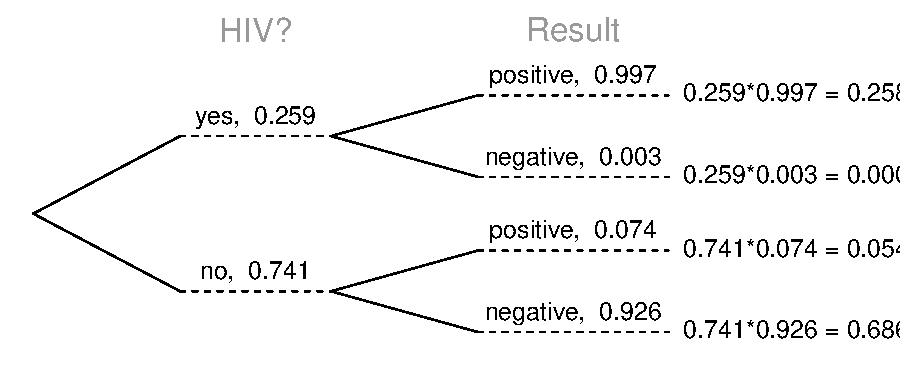
\includegraphics[width=60mm]{ch_probability_oi_biostat/figures/eoce/tree_hiv_swaziland/tree_hiv_swaziland.pdf}}

\textC{\end{multicols}
\newpage
\begin{multicols}{2}}


% 17

\eocesol{(a)~Let $E$ represent the event of agreeing with the idea of evolution and $D$ be the event of being a Democrat. From the problem statement, $P(E|D) = 0.67$. $P(E^C|D) = 1 - P(E|D) = 1 - 0.67 = 0.33$. \\
	(b)~Let $I$ represent the event of being an independent. $P(E|I) = 0.65$, as stated in the problem. \\
	(c)~Let $R$ represent the event of being a Republican. $P(E|R) = 1 - P(E^C|R) = 1 - 0.48 = 0.52$. \\
	(d)~0.35. $P(R|E) = \frac{P(E \textrm{ and }R)}{P(E)} = \frac{P(R)P(E|R)}{P(E)} = \frac{(0.40)(0.52)}{0.60} = 0.35$.}

% 18

\eocesol{(a)~Approximately 1,025 individuals would be expected to test positive; with approximately 25 true positive test results. The PPV of IRT is 0.0243.
	\\ $(100,000) P(T^+) = 100,000 [P(T+|D)P(D) + P(T|D^C)P(D^C)] = 100,000 [(0.87)(1/3500) + (1-0.99)(3499/3500)] \approx 1,025$. \\
	$(100,000) P(T^+|D) = (100,000)(0.87)(1/3500) \approx 25$. 
	$PPV \approx \frac{\textrm{\# true positives tests}}{\textrm{\# positive tests}} = 0.0243$. \\
	(b)~The PPV of IRT/IRT is 0.6839. Among the 1,025 individuals who tested positive in the first test, $25/1,025 = 0.0243$ are true positives; this represents the 'prevalence' of the group that undergo a second test. Recalculate PPV with the same test parameters: \\
	$PPV = \frac{P(T^+|D)P(D)}{P(T^+|D)P(D) + P(T^+|D^C)P(D^C)} = \\ \frac{(0.87)(0.0243)}{(0.87)(0.0243) + (1-0.99)(1-0.0243)} = 0.6839$.}

% 19

\eocesol{0.0714. Even when a patient tests positive for lupus, there is only a 7.14\% 
chance that he actually has lupus. House may be right.
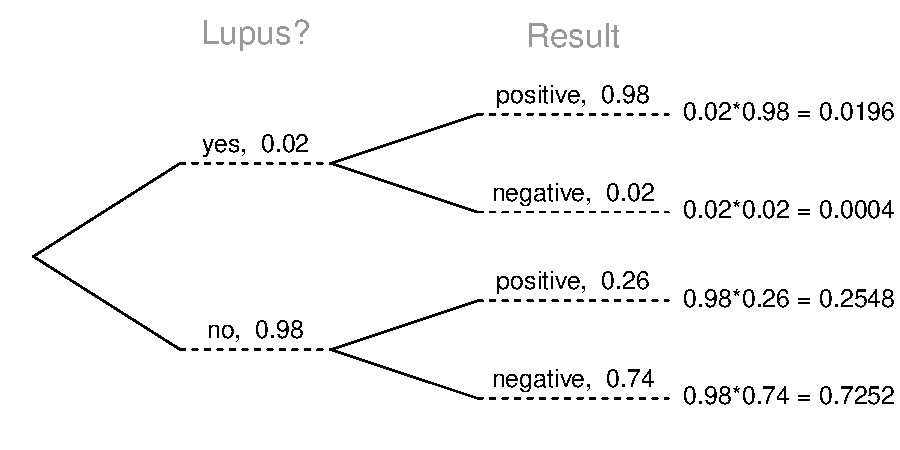
\includegraphics[width=60mm]{ch_probability_oi_biostat/figures/eoce/tree_lupus/tree_lupus.pdf}}


% 20

\eocesol{0.46. Let $I$ be the event of being identical twins, and $I^C$ be the event of being fraternal twins. Let $FF$ be the event that both twins are female. $P(I|FF) = \frac{P(I \textrm{ and } FF)}{P(FF)} = \frac{P(FF|I)P(I)}{P(FF|I)P(I) + P(FF|I^C)P(I^C)} = \frac{(0.50)(0.30)}{(0.50)(0.30) + (0.25)(1-0.30)} = 0.46$.\\
	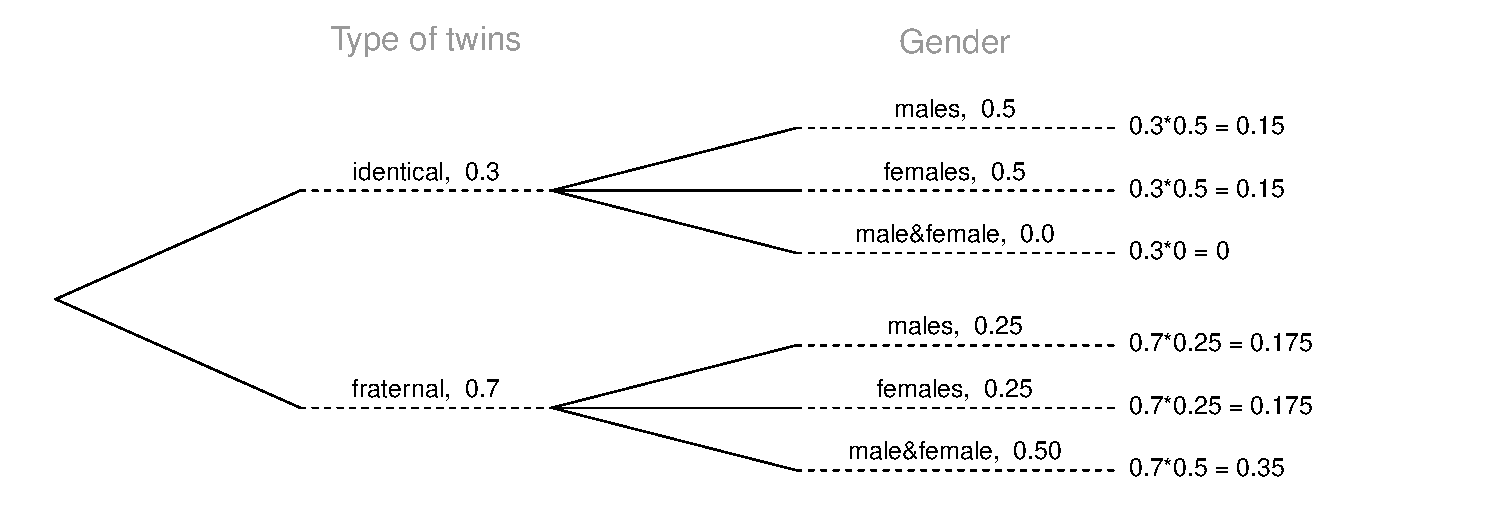
\includegraphics[width=60mm]{ch_probability_oi_biostat/figures/eoce/tree_twins/tree_twins.pdf}}

% 21

\eocesol{Mumps is the most likely disease state, since $P(B_3|A) = 0.563$, $P(B_1|A) = 0.023$, and $P(B_2|A) = .415$. $P(B_i|A) = \frac{P(A|B_i)P(B_i)}{P(A)}$. $P(A) = P(A \textrm{ and } B_1) + P(A \textrm{ and } B_2) + P(A \textrm{ and } B_3) = P(A|B_1)P(B_1) + P(A|B_2)P(B_2) + P(A|B_3)P(B_3)$. \\} 


% 22

\eocesol{(a)~In descending order on the table, the PPV for each age group is 0.070, 0.202, 0.293, 0.386, 0.403. As the prevalence of breast cancer increases, PPV also increases. If more women have the disease, the chance of a positive test result being a true positive increases (and the chances of the result being a false positive decreases). \\
	Consider the denominator, which quantifies the number of true positives and false positives. When prevalence increases, even though both the numerator and denominator are increasing from $[prev \times sensitivity]$, the denominator is also decreasing from $[(1-prev) \times (1-specificity)]$ decreasing (since as prevalence increases, the quantity $(1 - prev)$ decreases). Since sensitivity and specificity are constant, increasing prevalence has the effect of increasing the number of true positives (left term) and decreasing the number of false positives (right term). PPV increases when the number of true positives increases. \\
	(b)~ The technology that raises specificity to 99\% offers a higher increase. Since prevalence of the disease only ranges between less than 1\% to at most $\sim$ 4\%, most of the people tested do not have breast cancer. This implies that the low PPV is largely due to the high number of false positives. This value is related to the specificity. If specificity increases, this increases the number of true negatives and decreases the number of false positives. Increasing sensitivity can potentially increase the number of true positives detected and raise PPV, but this does not have as strong an effect.}

% 23 (oi_biostat)

\eocesol{(a)~Let $A$ be the event of knowing the answer and $B$ be the event of answering it correctly. Assume that if a participant knows the correct answer, they answer correctly with probability 1: $P(B|A) = 1$. If they guess randomly, they have 1 out of $m$ chances to answer correctly, thus $P(B|A^C) = 1/m$. $P(A|B)= \frac{1 \cdot p}{(1 \cdot p) +(\frac{1}{m} \cdot (1-p))} =  \frac{p}{p + \frac{1-p}{m}}$.  \\
	(b)~0.524. Let $A$ be the event of having an IQ over 150 and $B$ be the event of receiving a score indicating an IQ over 150. From the problem statement, $P(B|A) = 1$ and $P(B|A^C) = 0.001$. $P(A^C|B) = \frac{0.001 \cdot (1- \frac{1}{1,100})}{(1 \cdot (\frac{1}{1,100})) + (0.001 \cdot (1- \frac{1}{1,100}))} = 0.524$. }

% 24 (oi_biostat)

\eocesol{(a)~In descending order on the table, the PPV for each age group is 0.003, 0.064, 0.175, 0.270; the NPV for each age group is 0.999, 0.983, 0.948, 0.914.\\
	(b)~As prevalence of prostate cancer increases by age group, PPV also increases. However, with rising prevalence, NPV decreases.\\
	(c)~The probability that a man has prostate cancer, given a positive test, necessarily increases as the overall probability of having prostate cancer increases. If more men have the disease, the chance of a positive test result being a true positive increases (and the chances of the result being a false positive decreases). The decreasing NPV values follow similar logic: if more men have the disease, the chance of a negative test being a true negative decreases (and the chances of the result being a false negative increases).  \\
	(d)~Lowering the cutoff for a positive test would result in more men testing positive, since men with PSA values 2.5 ng/ml to 4.1 ng/ml were not previously classified as testing positive. Since the sensitivity of a test is the proportion who test positive among those who have disease, and the number with disease does not change, the proportion will increase, except in the rare and unlikely situation where the additional positive tests are among only men without the disease.}

%% 2.3 EXTENDED EXAMPLE

% 25 (oi_biostat)

\eocesol{(a)~Frequency of $X^+X^+$: 0.863. Frequency of $X^+X^-$: 0.132. Frequency of $X^-X^-$: 0.005. Frequency of $X^-Y$: 0.07. Frequency of $X^+Y$: 0.93. From frequency of $X^-X^-$, frequency of $X^-$ allele is $\sqrt{0.005} = 0.071$; thus, frequency of $X^+$ allele is $1 - 0.071 = 0.929$. Frequency of $X^+Y$ is $1 - 0.093 = 0.07$. \\
	(b)~0.033. Let $A$ be the event that two parents are not colorblind, and $B$ represent the event of having a colorblind child. On the tree, $\times$ represents a mating between two genotypes. $P(B|A) = [P(X^{+}X^{+} \times X^{+}Y| A) \cdot P(B |X^{+}X^{+} \times X^{+}Y)] + [P(X^{+}X^{-} \times X^{+}Y| A) \cdot P(B |X^{+}X^{-} \times X^{+}Y)] = (0.867)(0) + (0.133)(1/4) = 0.033$. \\
	\textit{\Tree [.A [.$X^{+}X^{+}$$\times$$X^{+}Y$ [ B $B^C$ ] ] [.$X^{+}X^{-}$$\times$$X^{+}Y$ [ B $B^C$ ] ] ]} \\
}


% 26 (oi_biostat)

\eocesol{(a)~1/9. Let $X$ represent the event of two parents having brown eyes and $Y$ represent the event of having a child with blue eyes. Solve for $P(Y|X)$. \\
	\textit{\Tree [.X [.BB$\times$BB [ Y $Y^C$ ] ] [.Bb$\times$Bb [ Y $Y^C$ ] ] [.BB$\times$Bb [ Y $Y^C$ ] ] ]} \\
	$P(Y|X) = [P(BB \times BB | X) \times P(Y| BB \times BB)] + [P(Bb \times Bb | X) \times P(Y| Bb \times Bb)] + [P(BB \times Bb | X) \times P(Y| BB \times Bb)]$\\
	Assuming independent mating, $P(BB \times BB | X) = 1/9$, $P(Bb \times Bb | X) = 4/9$, and $P(BB \times Bb | X) = 4/9$. $P(Y|X) = (1/9)(0) + (4/(9)(1/4) + (4/9)(0) = 1/9$.\\
	(b)~Yes, 1/6. $P(Bb \times Bb|X)$ is now 2/3, since $P(Bb |X, \textrm{paternal grandfather } bb) = 1$ for the father. \\
	(c)~ 3/32. Let $Y^C$ represent the event of having a first child with brown eyes, and $Z$ represent the event of having a second child with blue eyes. \\
	\textit{\Tree [.X,$Y^C$ [.BB$\times$BB Z $Z^C$ ]  [.Bb$\times$Bb Z $Z^C$ ] [.BB$\times$Bb Z $Z^C$ ] ]} \\
	Solve for $P(Z|X, Y^C)$. Only a $Bb \times Bb$ pairing can potentially produce a blue-eyed child, which simplifies the total probability equation to $P(Z|X, Y^C) = P(Bb \times Bb|X, Y^C)(1/4)$. Use Bayes' rule, then simplify: $P(Bb \times Bb|X, Y^C) = 3/8$. $P(Z|X, Y^C) = (3/8)(1/4) = 3/32 = 0.09375$.}


%_______________
\end{multicols}

\textC{\newpage}


%_______________
\eocesolch{Distributions of random variables}



%_______________
\begin{multicols}{2}

%% 3.1 RANDOM VARIABLES

% 1 (oi_biostat)
\eocesol{(a)~215 eggs. Let $X$ represent the number of eggs laid by one gull. $E(X) = 0.25(1) + 0.40(2) + 0.30(3) + 0.05(4) = 2.15.$ $E(100X) = 100E(X) = 215.$ \\
	(b)~85.29 eggs. $Var(X) = 0.25(1-2.15)^2 + 0.40(2-2.15)^2 + 0.30(3-2.15)^2 + 0.05(4-2.15)^2 = 0.7275.$ $Var(100X) = 100^2Var(X) = 7275 \rightarrow \sqrt{7275} = 85.29.$ }

% 2 

\eocesol{(a)~The probability of drawing three hearts equals $(13/52)(12/51)(11/50) = 0.0129$, and the probability of drawing three black cards equals $(26/52)(25/51)(24/50) = 0.1176$; thus, the probability of any other draw is $1 - 0.0129 - 0.1176 = 0.8694$. $E(X) = 0.0129(50) + 0.1176(25) + 0.8694(0) = 3.589.$ $Var(X) = 0.0129(50-3.589)^2 + 0.1176(25-3.589)^2 + 0.8694(0-3.589)^2 = 93.007$. $SD(X) = \sqrt{Var(X)} = 9.644.$ \\ (b)~Let $Y$ represent the net profit/loss, where $Y = X - 5$. $E(Y) = E(X - 5) = E(X) - 5 = -1.412$. Standard deviation does not change from a shift of the distribution; $SD(Y) = SD(X) = 9.644$. \\
	(c)~It is not advantageous to play, since the expected winnings are lower than \$5.}

% 3

\eocesol{(a)~$E(X) = \$12.7$. $SD(X) = \$14.08$. \\ (b)~$E(120X) = 120E(X) = \$1,524$. $SD(120X) = \sqrt{120^2Var(X)} = \$1689.45$. This calculation assumes that the amount of baggage each person checks is independent of each other. This may not be reasonable for a small number of passengers, since people traveling together may be likely to check a similar amount of baggage.}

% 4

\eocesol{(a)~$E(X + 3Y) = E(X) + 3E(Y) = 48 + 6 = 54 \textrm{ ounces}.$ $Var(X + 3Y) = Var(X) + 9Var(Y) = 1 + 9(0.0625) = 1.5625.$ $SD(X + 3Y) = 1.25$. \\(b)~$E(X - Y) = E(X) - E(Y) = 46 \textrm{ ounces}.$ $Var(X + Y) = Var(X) + Var(Y) = 1.0625$. $SD(X-Y) = 1.031$. \\ (c)~When either adding or removing a scoop of ice cream from a box, there is variability in the amount of ice cream scooped. Thus, variance is additive regardless of whether ice cream is added or removed.}

%% 3.2 BINOMIAL DISTRIBUTION

% 5

\eocesol{(a)~Binomial conditions are met: 
	(1)~Independent trials: In a random sample across the US, it is reasonable to assume that whether or not one 18-20 year old has consumed alcohol does not depend on whether or not another one has.
	(2)~Fixed number of trials: $n = 10$.
	(3)~Only two outcomes at each trial: Consumed or did not consume alcohol.
	(4)~Probability of a success is the same for each trial: $p = 0.697$. \\
	(b)~Let $X$ be the number of 18-20 year olds who have consumed alcohol; $X \sim \textrm{Bin}(10, 0.697)$. $P(X=6) = 0.203$. \\
	(c)~Let $Y$ be the number of 18-20 year olds who have not consumed alcohol; $Y \sim \textrm{Bin}(10, 1-0.697)$. $P(Y = 4) = P(X = 6) = 0.203$. \\
	(d)~$X \sim \textrm{Bin}(5, 0.697)$. $P(X \leq 2) =  0.167$. \\
	(e)~$X \sim \textrm{Bin}(5, 0.697)$. $P(X \geq 1) = 1 - P(X = 0) = 0.997$.}

% 6

\eocesol{(a)~Binomial conditions are met: 
	(1)~Independent trials: In a random sample across the US, it is reasonable to assume that whether or not one person has had chickenpox does not depend on whether or not another one has.
	(2)~Fixed number of trials: $n = 100$.
	(3)~Only two outcomes at each trial: Had or did not have chickenpox.
	(4)~Probability of a success is the same for each trial: $p = 0.90$. \\
	(b)~Let $X$ be the number of adults who have had chickenpox; $X \sim \textrm{Bin}(100, 0.90)$. $P(X=97) = 0.006$. \\
	(c)~Let $Y$ be the number of adults who have not had chickenpox; $Y \sim \textrm{Bin}(10, 1-0.90)$. $P(Y = 3) = P(X = 97) = 0.006$. \\
	(d)~$Y \sim \textrm{Bin}(10, 0.10)$. $P(Y \geq 1) =  1 - P(X=0) = 0.651$. \\
	(e)~$X \sim \textrm{Bin}(10, 0.90)$. $P(X \leq 7) = 0.070$.}

% 7

\eocesol{(a)~Both O+ and O- individuals can donate blood to a Type O+ patient; $n = 15$, $p = 0.45$. $\mu = np = 6.75$. $\sigma = \sqrt{np(1-p)} = 1.93$. \\
	(b)~Only O- individuals can donate blood to a Type O- patient; $n = 15$, $p = 0.08$. $P(X \geq 3) = 0.113$.}


% 8 

\eocesol{0.132. Let $X$ be the number of IV drug users who contract Hepatitis C within a month; $X \sim \textrm{Bin}(5, 0.30)$, $P(X = 3) = 0.132$.}

% 9

\eocesol{(a)~Let $X$ represent the number of infected stocks in the sample; $X \sim \textrm{Bin}(250, 0.30)$. $P(X = 60) = 0.006$. \\
	(b)~$P(X \leq 60) = 0.021$. \\
	(c)~$P(X \geq 80) = 0.735$. \\
	(D)~40\% of 250 is 100. $P(X \leq 100) = 0.997$. Yes, this seems reasonable; it is essentially guaranteed that within a sample of 250, no more than 40\% will be infected.}


% 10 

\eocesol{(a)~$(0.125)(1-0.125) = 0.109$. \\
	(b)~Let $X$ be the number of children with green eyes out of 2; $X \sim \textrm{Bin}(2, 0.125)$. $P(X = 1) = 0.219$. \\
	(c)~Let $Y$ be the number of children with green eyes out of 6; $Y \sim \textrm{Bin}(6, 0.125)$. $P(Y = 2 = 0.137)$. \\
	(d)$P(Y \geq 1) = 0.551$.}

% 11

\eocesol{(a)~$(200)(0.12) = 24$ cases of hyponatremia are expected during the marathon. \\
	(b)~Let $X$ represent the number of cases of hyponatremia during the marathon. $P(X > 30) = 0.082$.}


%% 3.3 NORMAL DISTRIBUTION

% 12

\eocesol{(a)~8.85\%.
	(b)~6.94\%.
	(c)~58.86\%.
	(d)~4.56\%. \\
	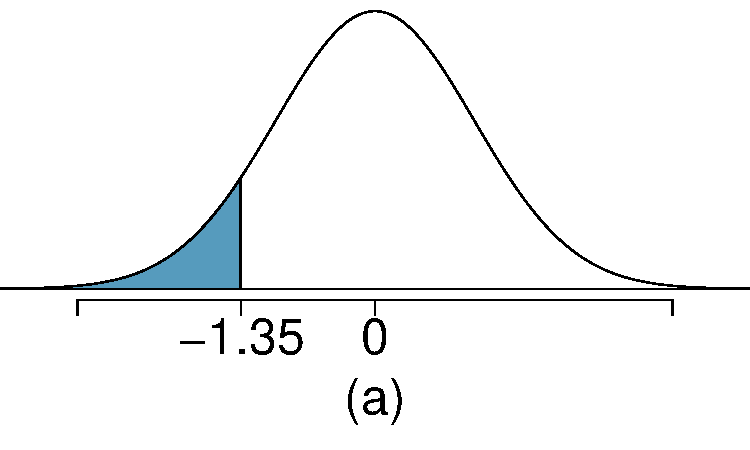
\includegraphics[width=0.23\textwidth]{ch_distributions_oi_biostat/figures/eoce/area_under_curve_1/zltNeg}
	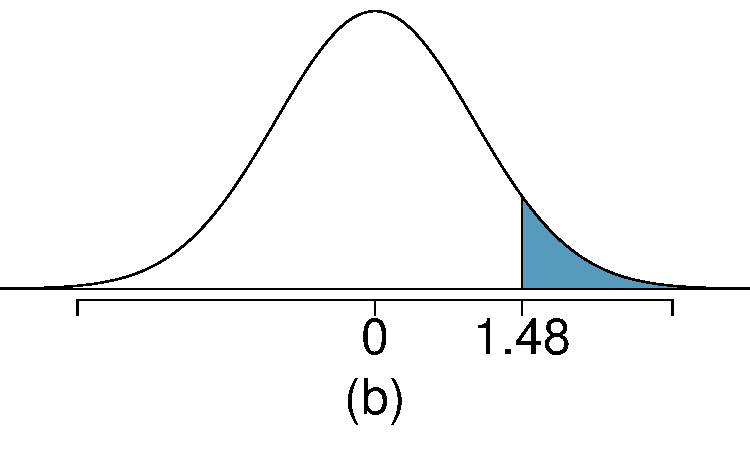
\includegraphics[width=0.23\textwidth]{ch_distributions_oi_biostat/figures/eoce/area_under_curve_1/zgtPos}
	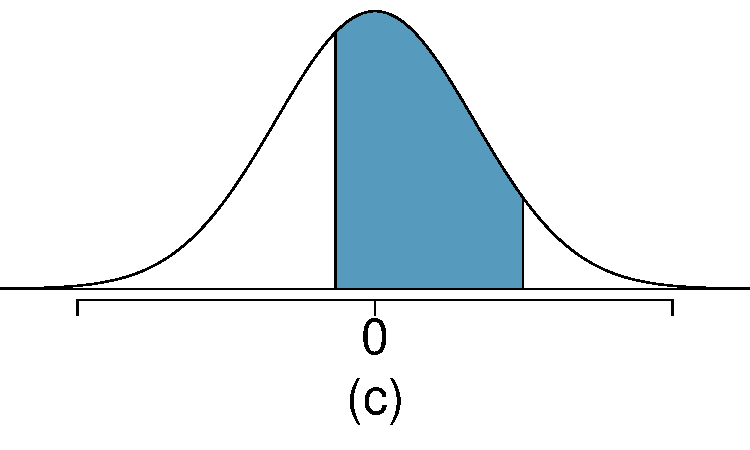
\includegraphics[width=0.23\textwidth]{ch_distributions_oi_biostat/figures/eoce/area_under_curve_1/zBet}
	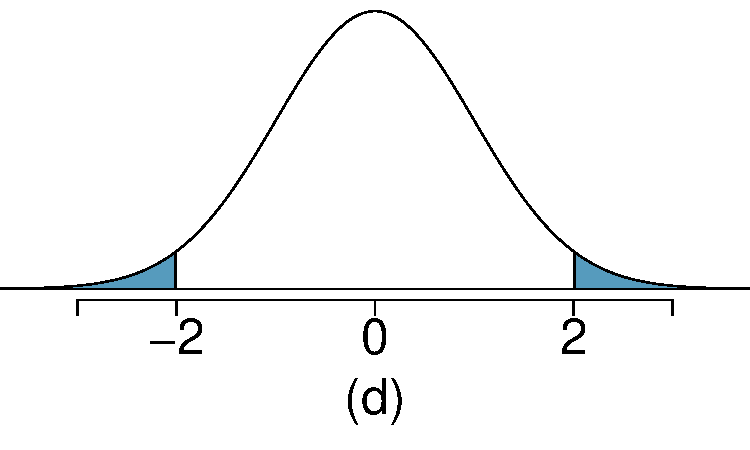
\includegraphics[width=0.23\textwidth]{ch_distributions_oi_biostat/figures/eoce/area_under_curve_1/zgtAbs}}

% 13

\eocesol{(a)~0.005. (b)~0.911. (c)~0.954. (d)~1.036. (e)~-0.842}

% 14

\eocesol{(a)~Verbal: $N(\mu = 151, \sigma = 7)$, Quant: $N(\mu = 153, \sigma = 7.67)$. $Z_{VR} = 1.29$, $Z_{QR} = 0.52$. She did better on the Verbal Reasoning section since her Z-score on that 
	section was higher.\\
	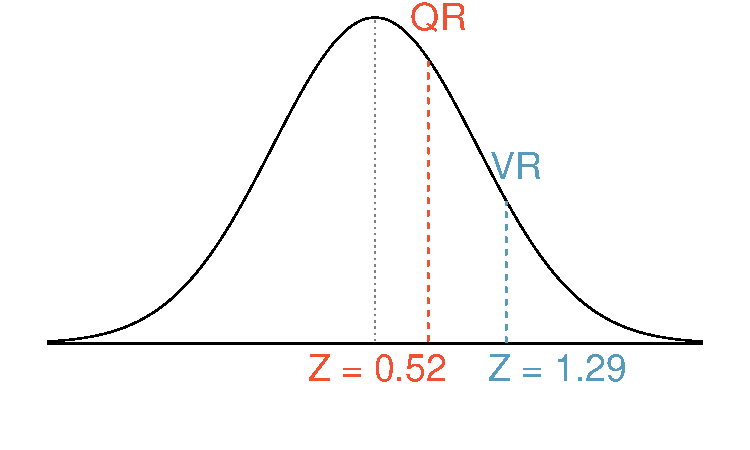
\includegraphics[width=0.3\textwidth]{ch_distributions_oi_biostat/figures/eoce/gre_intro/gre_intro.pdf} \\
	(b)~$Perc_{VR} = 0.9007 \approx 90\%$, $Perc_{QR} = 0.6990 \approx 70\%$. $100\% - 90\% = 10\%$ did better than her on VR, and $100\% - 70\% = 30\%$
	did better than her on QR. \\
	(c)~159.
	(d)~147.}

% 15

\eocesol{(a)~13.8\%. (b)~37.7\%. (c)~3,353 seconds. (d)~6,295 seconds.}

% 16

\eocesol{The tail area lower than -2.5 units on the standard normal curve equals 0.0062. Thus, .62\% of young adults suffer from osteoporosis according to this criterion.}


% 17

\eocesol{(a)~0.115. (b)~The coldest 10\% of days are colder than 70.59\degree F.}


% 18

\eocesol{(a)~0.099. (b)~The largest 5\% of egg clutches have volume of more than 1507.5 mm$^3$. }

% 19

\eocesol{(a)~0.023. (b)~72.66 mg/dL.}

% 20

\eocesol{The middle 95\% of this distribution is defined by 0.260 and 6.140 $\mu$g/dl.}

% 21

\eocesol{(a)~82.4\%. (b)~About 38 years of age.}

% 22

\eocesol{(a)~$\frac{x-\mu}{\sigma} = Z$. $\sigma = 15.58$. (b)~39.04 mg/dL.}

% 23

\eocesol{Let $A$ be the event of scoring above 2100 and $B$ be the event of scoring above 1900. The question asks for $P(A|B)$. By the definition of conditional probability, $P(A|B) = \frac{P(A \textrm{ and } B)}{P(B)}$. In the context of this question, $P(A \textrm{ and } B = P(A)$, since if someone scores above 2100, they necessarily score above 1900. $P(A) = 0.023$, $P(B) = 0.091$. $P(A|B) = 0.249$. }

% 24

\eocesol{(a)~$n = 50$, and $p = 0.70$. $\mu = np = 35$. $\sigma = \sqrt{np(1-p)} = 3.24$. \\
	(b)~Both $np$ and $n(1-p)$ are greater than 10. Thus, it is valid to approximate the distribution as $X \sim N(35, 3.24)$, where $X$ is the number of 18-20 year olds who have consumed alcohol. $P(X \geq 45) = 0.001$. }

% 25

\eocesol{(a)~$n = 120$, and $p = 0.90$.  $\mu = np = 108$. $\sigma = \sqrt{np(1-p) = 3.29}$. \\
	(b)~Both $np$ and $n(1-p)$ are greater than 10. Thus, it is valid to approximate the distribution as $X \sim N(108, 3.29)$, where $X$ is the number of adults who have had chickenpox as a child. $P(X \leq 105) = 0.181$.}

% 26

\eocesol{Let $X$ represent the number of students who accept the the offer; $X \sim \textrm{Bin}(2500, 0.70)$. This distribution can be approximated by a $N(1750, 22.91)$. The approximate probability that the school does not have enough dorm room spots equals $P(X \geq 1,786) = 0.06$.}

% 27

\eocesol{The data appear to follow a normal distribution, since the points closely follow the line on the normal probability plot. There are some small deviations, but this is to be expected for such a small sample size.}


%% 3.4 POISSON DISTRIBUTION

% 28 

\eocesol{(a)~$P(X = 2) = \frac{\exp^{-2}(2^2)}{2!} = 0.271$. (b)~$P(X \leq 2) = P(X = 0) + P(X = 1) + P(X = 2) = 0.677$. (c)~$P(X \geq 3) = 1 - P(X \leq 2) = 0.323$.}

% 29

\eocesol{(a)~$\lambda = 1$; thus $\mu = \lambda = 1$ and $\sigma = \sqrt{\lambda} = 1$. (b)~Let $X$ represent the number of typos made in an hour. $P(X \leq 3) = 0.981$. (c)~Let $Y$ represent the number of typos made in 3 hours; $\lambda = 1$, $t = 3$. $P(Y \geq 5) = 0.185$. }

% 30

\eocesol{(a)~$p = \frac{8}{10^6}$, $n = 1.4 \times 10^6$. $\lambda = np = 11.2$ The expected number of cases in a given year is 11.2\\
	(b)~$P(X \geq 15) = 1 - P(X \leq 14) = 0.161$. \\
	(c)~For Brooklyn, $\lambda = 3.6$. The probability of 10 or more cases in Brooklyn in a given year is 0.004. }

% 31 

\eocesol{(a)~$\lambda$ for a population of 2,000,000 male births is 400. The probability of at most 380 newborn males with hemophilia is $P(X \leq 380$), where $X \sim \textrm{Pois}(400)$: 0.165. \\
	(b)~$P(X \geq 450) = 0.0075$. \\
	(c)~The number of male births is (1/2)(1,500,000) = 750,000. The rate $\lambda$ for one year is 150. Over 5 years, the rate $\lambda$ is 750. The expected number of hemophilia births over 5 years is 750 and the standard deviation is $\sqrt{750} = 27.39$.}

% 32

\eocesol{(a)~The number of non-Hispanic whites is $(769,000)(0.73) = 561,370$; $\lambda$ = $(6.8/100,000)(561,370) = 38.17$. $P(X \geq 146) = 2.62 \times 10^{-40}$. \\
	(b)~To compute the observed rate in terms of deaths per 100,000 non-Hispanic whites, divide the number of overdose fatalities reported by the total number of non-Hispanic whites, and multiply by 100,000 $\rightarrow$ $(146,000/561,370)(100,000) = 26.0078$. \\
	(c)~The observed rate $\lambda$ is simply 146, since the population did not change. $P(X \geq 165) = 0.065$.}

%% 3.5 DISTRIBUTIONS RELATED TO BERNOULLI TRIALS

% 33

\eocesol{(a)~On average, 2 women would need to be sampled in order to select a married woman ($\mu = 1/p = 2.123$), with standard deviation 1.544 ($\sigma = \sqrt{\frac{(1-p)}{p^2}}$). \\
	(b) $\mu = 3.33$. $\sigma = 2.79$. \\
	(c)~Decreasing the probability increases both the mean and the standard deviation. }

% 34 
\eocesol{(a)~On average, about 3 donors would need to be sampled before selecting a Type O+ individual ($\mu = 2.70$), with standard deviation 2.15. \\
	(b)~Let $X$ represent the number of donors that must be sampled to find a Type O+ individual; $X \sim \textrm{Geom}(0.37)$. $P(X = 4) = 0.093$. \\
	(c)~$P(X > 4) =  0.158$. \\
	(d)~Let $Y$ represent the number of donors that must be sampled to find a Type O- individual; $Y \sim \textrm{Geom}(0.08)$. $P(Y \leq 4) = 0.284$. \\
	(e)~$\mu = 12.5$, $\sigma = 11.99$. \\
	(f)~$P(Y \leq 3) = 0.221$.}

% 35

\eocesol{(a)~Let $X$ represent the number of stocks that must be sampled to find an infected stock; $X \sim \textrm{Geom}(0.30)$. $P(X \leq 5) = 0.832$.\\
	(b)~$P(X \leq 6) = 0.882$.\\
	(c)~$P(X \geq 3) = 1 - P(X \leq 2) = 0.49$. }

% 36 

\eocesol{(a)~0.142, negative binomial with $r = 10$, $p = 0.65$.\\
	(b)~0.212, binomial with $n = 15$, $p = 0.65$.\\
	(c)~0.080, geometric with $p = 0.65$. }

% 37 

\eocesol{(a)~0.102, geometric with $p = 1994/14,604 = 0.137$.\\
	(b)~0.854, binomial with $n = 10$, $p = 0.137$.\\
	(c)~0.109, binomial with $n = 10$, $p = 0.137$.\\
	(d)~The mean and standard deviation of a negative binomial random variable with $r = 4$ and $p = 0.137$ are 29.30 and 13.61, respectively.}

% 38

\eocesol{(a)~0.04, negative binomial with $r = 3$, $p = 0.15$.\\
	(b)~Since the trials are independent, the probability of making the next serve is 0.15.\\
	(c)~The first scenario is a probability statement about 3 successful serves occurring with 10 trials; the second, however, is only asking about the next serve.}

% 39

\eocesol{(a)~$\mu = 2.05$; $\sigma^2 = 1.77$. \\
	(b)~Let $X$ represent the number of soapy-taste detectors; $X \sim \textrm{HGeom}(1994, 14604-1994,15)$. $P(X = 4) = 0.09435$.\\
	(c)~$P(X \leq 2) = 0.663$.\\
	(d)~0.09437, from the binomial distribution. With a large sample size, sampling with replacement is highly unlikely to result in any particular individual being sampled again. In this case, the hypergeometric and binomial distributions will produce equal probabilities.}

% 40

\eocesol{(a)~0.664, binomial with $n = 7$, $p = 0.44$.\\
	(b)~0.246, geometric with $p = 0.44$.\\
	(c)~0.022, hypergeometric with $m = 350-154$, $N-m = 154$, $n = 10$. \\
	(d)~0.030, binomial with $n = 50$, $p = 0.44$.\\}



\textC{}
\end{multicols}
\newpage


%%%%%%%%%%%%%%%%%%%%%%%%%%%%%%%%%%%%%%%%%%%%%%%%%%%%%%%%%%%%%%%%%%%%%%%%%%%%%%%%%%%%%%%%%%%%%%%%%%%%%%%%%%%%%%

%_______________
\eocesolch{Foundations for inference}



%_______________
\begin{multicols}{2}

%% 4.1 SAMPLING VARIABILITY

% 1

\eocesol{(a)~$\overline{x} = 171.1$. \\
	(b)~$s = 9.4$. IQR: $177.8-163.8 = 14$. \\
	(c)~$Z_{180} = \frac{180-171.1}{9.4} = 0.94$. A height of 180 cm is not considered unusually tall, since it is within 2 SD of the mean.
	$Z_{155} = \frac{155-171.1}{9.4} = -1.71$. A height of 155 cm is not considered unusually short, since it is within 2 SD of the mean. \\
	(d) No, due to sampling variation between samples, it is likely that the mean and standard deviation of the new sample will differ from 171.1 and 9.4. \\
	(e) The standard error of the sample mean is given by $\frac{s}{\sqrt{n}} = \frac{9.4}{\sqrt{507}} = 0.417$. \\
	}

% 2 (oi biostat)

\eocesol{(a)~$\overline{x} = 0.6052.$ \\
	(b)~$s = 0.0131$. \\
	(c)~$Z_{0.63} = \frac{0.63 - 0.6052}{0.0131} = 1.893$. No, this level of BGC is within 2 SD of the mean. \\
	(d)~The standard error of the sample mean is given by $\frac{s}{\sqrt{n}} = \frac{0.0131}{\sqrt{70}} = 0.00157$.
	}

% 3 (oi)

\eocesol{(a)~This is the sampling distribution of the sample mean. \\
(b)~The sampling distribution will be normal and symmetric, centered around the theoretical population mean $\mu$ of the number of eggs laid by this hen species during a breeding period. \\
(c)~The variability of the distribution is the standard error of the sample mean:  $\frac{s}{\sqrt{n}} = \frac{18.2}{\sqrt{45}} = 2.71$. \\
(d)~The variability of the new distribution will be greater than the variability of the original distribution. Conceptually, a smaller sample is less informative, which leads to a more uncertain estimate. This can be shown concretely with a calculation: $\frac{18.2}{\sqrt{10}} = 5.76$ is larger than 2.71.
}


%% 4.2 CONFIDENCE INTERVALS

% 4 (oi)

\eocesol{A 95\% CI for the proportion of U.S. adults who live with one or more chronic conditions is $0.45 \pm (1.96 \times 0.012) = (0.43, 0.47).$ With 95\% confidence, the proportion of U.S. adults who live with one or more chronic conditions is contained within the interval (0.43, 0.47).
}

% 5 (oi)

\eocesol{A 99\% CI for the proportion of U.S. adult Twitter users who get at least some news on Twitter is $0.52 \pm (2.58 \times 0.024) = (0.46, 0.58).$ With 99\% confidence, the proportion of U.S. adult Twitter users who get at least some news on Twitter is contained within the interval (0.46, 0.58).
	}

% 6 (oi)

\eocesol{(a)~False. Due to sampling variability, there is a chance the confidence interval does not contain the population parameter $\mu$. \\
	(b)~True. This is the definition of a confidence interval. \\
	(c)~True. The 95\% confidence interval does not contain 0.50 and is lower than 0.50; this corresponds to a test at the $\alpha = 0.05$ level.\\
	(d)~False. The standard error represents the variability of the point estimate, not the uncertainty of respondents.
	}
	
% 7 (oi)

\eocesol{(a)~False. The value 0.50 is contained within the 99\% confidence interval. There is not statistically significant evidence that more than half of U.S. adult Twitter users get some news through Twitter. \\
	(b)~False. The standard error represents the variability of the point estimate and is not a measure of study participation. \\
	(c)~False. Reducing the standard error requires collecting more data (i.e., increasing $n$). \\
	(d)~False. A 90\% confidence interval is less wide than a 99\% confidence interval.
	}

% 8 (oi, edited)

\eocesol{(a)~We are 95\% confident that the mean number of hours that U.S. residents have to relax or pursue activities that they enjoy is between 3.53 and 3.83 hours. \\
	(b)~A larger margin of error with the same sample occurs with a higher confidence level (i.e., larger critical value). \\
	(c)~The margin of error will be smaller, since $n$ has increased. \\
	(d)~A 90\% confidence interval will be smaller than the original 95\% interval, since the critical value is smaller and results in a smaller margin of error. The interval will provide a more precise estimate, but have an associated lower confidence of capturing $\mu$.
}

% 9 (oi, edited)

\eocesol{(a)~The mean number of days US residents experienced poor mental health during the past 30 days is contained within the interval (3.40, 4.24) days. \\
	(b)~In this context, 95\% confident implies that 950 out of 1,000 intervals constructed are expected to contain the true mean number of days US residents experienced poor mental health during the past 30 days. \\
	(c)~A 99\% interval will be larger than the 95\% confidence interval. \\
	(d)~The standard error of the estimate would be larger, since 500 individuals is fewer than 1,151 individuals. Reducing sample size increases the standard error.
	}

% 10 (oi, edited)

\eocesol{(a)~False. Provided the data distribution is not very strongly skewed ($n = 64$ in 
this sample, so we can be slightly lenient with the skew), the distribution of the sample mean will 
be nearly normal, allowing for the normal approximation. \\
(b)~False. Inference is made on the population parameter, not the point 
estimate. The point estimate is always in the confidence interval. \\
(c)~True. \\
(d)~False. The confidence interval is not about a sample mean. \\
(e)~False. A wider interval is required to be more confident about capturing the parameter. \\
(f)~True. The margin of error is half the width of the interval, 
and the sample mean is the midpoint of the interval. \\
(g)~False. To halve the margin of 
error requires sampling $2^2 = 4$ times the number of people in 
the initial sample.}

% 11 (oi, edited)

\eocesol{(a)~False. Inference is not made about the sample. \\
	(b)~False. The data are not strongly skewed, and the distribution of the sample mean will be nearly normal. \\
	(c)~False. Confidence intervals are not about sample means. \\
	(d)~True. \\
	(e)~True. \\
	(f)~True.
	}


% 12 (oi, edited)

\eocesol{The normal approximation is valid; the distribution of the sample mean is nearly normal. The 95\% confidence interval is $23.44 \pm (1.96 \times \frac{4.72}{sqrt{5534}}) = (23.31, 23.56)$. The mean age of first marriage for women in the US is contained by the interval (23.31, 23.56) years. Note that this assumes the sample collected by the CDC is representative of all US women.}

%% 4.3 HYPOTHESIS TESTING


% 13 (oi)

\eocesol{(a)~The null hypothesis is that New Yorkers sleep an average of 8 hours of night ($H_0: \mu = 8$ hours). The alternative hypothesis is that New Yorkers sleep less than 8 hours a night on average ($H_A: \mu < 8$ hours). \\
	 (b)~The null hypothesis is employees spend on average 15 minutes on non-business activities in a day ($H_0: \mu = 15$ minutes). The alternative hypothesis is that employees spend on average more than 15 minutes on non-business activities in a day ($H_A: \mu > 15$ minutes).
	}

% 14 (oi)

\eocesol{(a)~The null hypothesis is that the average calorie intake of diners is 1,100 calories ($H_0: \mu = 1,100$ calories). The alternative hypothesis is that average calorie intake of diners differs from 1,100 calories ($H_A: \mu \neq 1,100$ calories). \\
	(b)~The null hypothesis is that the average verbal reasoning score is 462 ($H_0: \mu = 462$ points). The alternative hypothesis is that the average verbal reasoning score is different from 462 ($H_A: \mu \neq 462$ points).
	}

% 15 (oi)

\eocesol{Hypotheses are always made about the population parameter $\mu$, not the sample mean $\overline{x}$. The correct value of $\mu_0$ is 10 hours, as based on the previous evidence; both hypotheses should include $\mu_0$. The correct hypotheses are $H_0: \mu = 10$ hours and $H_A: \mu > 10$ hours. 
	} 

% 16 (oi)

\eocesol{Hypotheses are always made about the population parameter $\mu$, not the sample mean $\overline{x}$. Since the scientist is interested in a difference in either direction, the alternative hypothesis should be two-sided. The correct hypotheses are $H_0: \mu = 23.44$ years and $H_A: \mu \neq 23.44$ years.
	}

% 17 (oi)

\eocesol{(a)~This claim is not supported by the confidence interval. 3 hours corresponds to a time of 180 minutes; there is evidence that the average waiting time is lower than 3 hours. \\
	(b)~2.2 hours corresponds to 132 minutes, which is within the interval. It is plausible that $\mu$ is 132 minutes, since we are 95\% confident that the interval (128 minutes, 147 minutes) contains the average wait time. \\
	(c)~Yes, the claim would be supported based on a 99\% interval, since the 99\% interval is wider than the 95\% interval.
	}

% 18 (oi)

\eocesol{$H_0: \mu = 130$ grams, $H_A: \mu \neq 130$ grams. Test the hypothesis by calculating the test statistic: $t = \frac{\overline{x} - \mu_0}{s/\sqrt{n}} = \frac{130 - 134}{17/sqrt{35}} = 1.39$. This results in a $p$-value of 0.17. There is insufficient evidence to reject the null hypothesis. There is no evidence that the nutrition label does not provide an accurate measure of calories.
	}

% 19 (oi)

\eocesol{(a)~Yes. The data are approximately symmetric, the sample size is large enough to support using the normal approximation, and it is reasonable to assume independence. \\
	(b)~$H_0: \mu = 32$ months, $H_A: \mu < 32$ months. Calculate the test statistic: $t = \frac{\overline{x} - \mu_0}{s/\sqrt{n}} = \frac{30.69 - 32}{4.31/\sqrt{36}} = -1.82$. The $p$-value is 0.08. There is sufficient evidence at the $\alpha = 0.10$ level to reject the null hypothesis and accept the alternative that the mean age at which gifted children count to 10 is lower than in the general population. \\
	(c)~Under the null hypothesis (if the mean age at which gifted children count to 10 equals 32 months), the probability of observing data as or more extreme as these is 0.08. \\
	(d)~The 90\% confidence interval is $\overline{x} \pm (1.65 \times s/\sqrt{n}) = (29.50, 31.88)$ months.
	(e)~Yes, the results from the test and confidence interval agree. The 90\% confidence interval does not contain $\mu_0$ of 32 months, and is shifted lower than $\mu_0$. 
	}

% 20 (oi)

\eocesol{(a)~Yes, the change in wait times is statistically significant at the $\alpha = 0.05$ level; the 95\% confidence interval does not contain 127 minutes. The 95\% interval is $137.5 \pm (1.96 \times 39/\sqrt{64}) = (127.95, 147.06)$ minutes. \\
	(b)~If the significance level were changed to $\alpha = 0.01$, then there would not be sufficient evidence to reject $H_0: \mu = 127$ minutes. There would not be sufficient evidence to suggest the wait times have changed. The 99\% confidence interval is (124.92, 150.08) minutes.\\
	(c)~At the $\alpha = 0.05$ significance level, there is evidence to suggest the average wait time in the ER has increased. However, this is not necessarily due to oversight on the hospital administrator's part; other factors may be at work. For example, perhaps increased wait times are due to more patients checking into the ER this year than last year. Alternatively, a sample size of 64 is relatively small, and it is certainly possible that extreme outliers may have overly influenced the mean. It would be advisable to take a closer look at the data distribution or repeat the test once more data have been collected.
	}

% 21 (oi)

\eocesol{(a)~$H_0: \mu = 100$, $\mu \neq 100$. Calculate the test statistic: $t = \frac{\overline{x} - \mu_0}{s/\sqrt{n}} = \frac{118.2-100}{6.5/\sqrt{36}} = 3.03$. The $p$-value is 0.0045. There is sufficient evidence that the mean IQ of mothers of gifted children is different from 100; based on $\overline{x}$, these data provide evidence that the mean IQ of mothers of gifted children is higher than 100. \\
	(b)~The 90\% confidence interval is $118.2 \pm (1.65 \times 6.5/\sqrt{36}) = (108.3, 128.1)$. \\
	(c)~Yes, the results agree. The 90\% confidence interval does not contain 100, and is shifted higher than 100. 
	}

% 22 (oi biostat)

\eocesol{(a)~The 95\% confidence interval is $3,150 \pm (1.96 \times 250/\sqrt{50}) = (3080.7, 3219.3)$ grams. \\
	(b)~She will conduct a test of the null against the two-sided alternative $H_A: \mu \neq 3250$ grams. Calculate the test statistic: $t = \frac{\overline{x} - \mu_0}{s/\sqrt{n}} = \frac{3150 - 3250}{250/\sqrt{50}} = -2.83$. The $p$-value is 0.007. There is sufficient evidence to reject the null hypothesis and conclude that the mean birthweight of babies from inner-city teaching hospitals is lower than 3,260 grams.
	}

% 23 (oi)

\eocesol{(a)~$H_0$: Anti-depressants do not help symptoms of fibromyalgia. $H_A$: Anti-
depressants do treat symptoms of fibromyalgia. 
(b)~Concluding that anti-depressants work for the treatment of fibromyalgia 
symptoms when they actually do not.
(c)~Concluding that anti-depressants do not work for the treatment of 
fibromyalgia symptoms when they actually do.
(d) If she makes a Type 1 error, she will continue taking medication that does not actually treat her disorder. If she makes a Type 2 error, she will stop taking medication that could treat her disorder.}

% 24 (oi)

\eocesol{(a)~$H_0$: The restaurant is meeting regulations. $H_A$: The restaurant is not meeting regulations (i.e., sanitation practices are poorer than required). \\
	(b)~A Type I error is concluding the restaurant is not meeting regulations when they are. \\
	(c)~A Type II error is concluding the restaurant is meeting regulations when they are not. \\
	(d)~A Type I error is more problematic for the restaurant, since they will lose the license to serve food even when they are meeting regulations. \\
	(e)~A Type II error is more problematic for diners, because they will be in danger of being served food that is not prepared in sanitary conditions. \\
	(f)~As a diner, I would prefer that the inspector requires strong evidence of health concerns rather than very strong before revoking a license, because a Type II error is more dangerous to public health. 
	}

% 25 (oi)

\eocesol{(a)~The standard error is larger under scenario I; standard error is larger for smaller values of $n$. \\
	(b)~The margin of error is larger under scenario I; to be more confidence of capturing the population parameter requires a larger confidence interval. \\
	(c)~The $p$-value from a Z-statistic only depends on the value of the Z-statistic; the value is equal under the scenarios. \\
	(d)~The probability of making a Type II error and falsely rejecting the alternative is higher under scenario I; it is easier to reject the alternative with a high $\alpha$.  
	}

% 26 (oi)

\eocesol{(a)~True. The 99\% confidence interval is wider than the 95\% confidence interval. \\
	(b)~False. Decreasing the significance level decreases the probability of making a Type I error. \\
	(c)~False. Failing to reject $H_0$ does not imply that $H_0$ is true. \\
	(d)~False. The probability of making a Type II error and the power of a test, by definition, must sum to 1; this is not related to whether or not the alternative is true. \\
	(e)~True. With large sample sizes, the standard error is very small and results in large test statistics (and hence, small $p$-values).
	}

\end{multicols}



%%%%%%%%%%%%%%%%%%%%%%%%%%%%%%%%%%%%%%%%%%%%%%%%%%%%%%%%%%%%%%%%%%%%%%%%%%%%%%%%%%%%%%%%%%%%%%%%%%%%%%%%%%%%%%
%\begin{comment}




\eocesolch{Inference for numerical data}


\begin{multicols}{2}

% 1
\eocesol{(a)~$df=6-1=5$, $t_{5}^{\star} = 2.02$ (column with two tails of 0.10, row with $df=5$).
(b)~$df=21-1=20$, $t_{20}^{\star} = 2.53$ (column with two tails of 0.02, row with $df=20$).
(c)~$df=28$, $t_{28}^{\star} = 2.05$.
(d)~$df=11$, $t_{11}^{\star} = 3.11$.}

% 3
\eocesol{(a)~between 0.025 and 0.05
(b)~less than 0.005
(c)~greater than 0.2
(d)~between 0.01 and 0.025}

% 5
\eocesol{The mean is the midpoint: $\bar{x} = 20$. Identify the margin of error: $ME = 1.015$, then use $t^{\star}_{35} = 2.03$ and $SE=s/\sqrt{n}$ in the formula for margin of error to identify $s = 3$.}

% 7
\eocesol{(a)~$H_0$: $\mu = 8$ (New Yorkers sleep 8 hrs per night on average.) $H_A$: $\mu < 8$ (New Yorkers sleep less than 8 hrs per night on average.)
(b)~Independence: The sample is random and from less than 10\% of New Yorkers. The sample is small, so we will use a $t$-distribution. For this size sample, slight skew is acceptable, and the min/max suggest there is not much skew in the data. $T = -1.75$. $df=25-1=24$.
(c)~$0.025 <$ p-value $<0.05$. If in fact the true population mean of the amount New Yorkers sleep per night was 8 hours, the probability of getting a random sample of 25 New Yorkers where the average amount of sleep is 7.73 hrs per night or less is between 0.025 and 0.05.
(d)~Since p-value $<$ 0.05, reject $H_0$. The data provide strong evidence that New Yorkers sleep less than 8 hours per night on average.
(e)~No, as we rejected $H_0$.}

% 9
\eocesol{$t^{\star}_{19}$ is 1.73 for a one-tail. We want the lower tail, so set -1.73 equal to the T-score, then solve for $\bar{x}$: 56.91.}


\textC{
\end{multicols}
\newpage
\begin{multicols}{2}
}


% 11
\eocesol{(a)~We will conduct a 1-sample $t$-test. $H_0$: $\mu = 5$. $H_A$: $\mu < 5$. We'll use $\alpha = 0.05$. This is a random sample, so the observations are independent. To proceed, we assume the distribution of years of piano lessons is approximately normal. $SE = 2.2 / \sqrt{20} = 0.4919$. The test statistic is $T = (4.6 - 5) / SE = -0.81$. $df = 20 - 1 = 19$. The one-tail p-value is about 0.21, which is bigger than $\alpha = 0.05$, so we do not reject $H_0$. That is, we do not have sufficiently strong evidence to reject Georgianna's claim. \\
(b)~Using $SE = 0.4919$ and $t_{df = 19}^{\star} = 2.093$, the confidence interval is (3.57, 5.63). We are 95\% confident that the average number of years a child takes piano lessons in this city is 3.57 to 5.63 years. \\
(c)~They agree, since we did not reject the null hypothesis and the null value of 5 was in the $t$-interval.}

% 13
\eocesol{If the sample is large, then the margin of error will be about $1.96 \times 100 / \sqrt{n}$. We want this value to be less than 10, which leads to $n \geq 384.16$, meaning we need a sample size of at least 385 (round up for sample size calculations!).}

% 15
\eocesol{(a)~Two-sided, we are evaluating a difference, not in a particular direction.
(b)~Paired, data are recorded in the same cities at two different time points. The temperature in a city at one point is not independent of the temperature in the same city at another time point.
(c)~$t$-test, sample is small and population standard deviation is unknown.
}

% 17
\eocesol{(a)~Since it's the same students at the beginning and the end of the semester, there is a pairing between the datasets, for a given student their beginning and end of semester grades are dependent.
(b)~Since the subjects were sampled randomly, each observation in the men's group does not have a special correspondence with exactly one observation in the other (women's) group.
(c)~Since it's the same subjects at the beginning and the end of the study, there is a pairing between the datasets, for a subject student their beginning and end of semester artery thickness are dependent.
(d)~Since it's the same subjects at the beginning and the end of the study, there is a pairing between the datasets, for a subject student their beginning and end of semester weights are dependent.}

% 19
\eocesol{(a)~For each observation in one data set, there is exactly one specially-corresponding observation in the other data set for the same geographic location. The data are paired.
(b)~$H_0: \mu_{diff} = 0$ (There is no difference in average daily high temperature between January 1, 1968 and January 1, 2008 in the continental US.) $H_A: \mu_{diff} > 0$ (Average daily high temperature in January 1, 1968 was lower than average daily high temperature in January, 2008 in the continental US.) If you chose a two-sided test, that would also be acceptable. If this is the case, note that your p-value will be a little bigger than what is reported here in part~(d).
(c)~Independence: locations are random and represent less than 10\% of all possible locations in the US. The sample size is at least 30. We are not given the distribution to check the skew. In practice, we would ask to see the data to check this condition, but here we will move forward under the assumption that it is not strongly skewed.
(d)~$Z=1.60$ $\to$ p-value $=0.0548$.
(e)~Since the p-value $> \alpha$ (since not given use 0.05), fail to reject $H_0$. The data do not provide strong evidence of temperature warming in the continental US. However it should be noted that the p-value is very close to 0.05.
(f)~Type~2 Error, since we may have incorrectly failed to reject $H_0$. There may be an increase, but we were unable to detect it.
(g)~Yes, since we failed to reject $H_0$, which had a null value of 0.}

% 21
\eocesol{(a)~(-0.03, 2.23).
(b)~We are 90\% confident that the average daily high on January 1, 2008 in the continental US was 0.03 degrees lower to 2.23 degrees higher than the average daily high on January 1, 1968.
(c)~No, since 0 is included in the interval.}


\textC{
\end{multicols}
\newpage
\begin{multicols}{2}
}


% 23
\eocesol{(a)~Each of the 36 mothers is related to exactly one of the 36 fathers (and vice-versa), so there is a special correspondence between the mothers and fathers.
(b)~$H_0: \mu_{diff} = 0$. $H_A: \mu_{diff} \ne 0$. Independence: random sample from less than 10\% of population. Sample size of at least 30. The skew of the differences is, at worst, slight. $Z = 2.72$ $\to$ p-value $= 0.0066$. Since p-value $<$ 0.05, reject $H_0$. The data provide strong evidence that the average IQ scores of mothers and fathers of gifted children are different, and the data indicate that mothers' scores are higher than fathers' scores for the parents of gifted children.}

% 25
\eocesol{No, he should not move forward with the test since the distributions of total personal income are very strongly skewed. When sample sizes are large, we can be a bit lenient with skew. However, such strong skew observed in this exercise would require somewhat large sample sizes, somewhat higher than~30.}

% 27
\eocesol{(a)~These data are paired. For example, the Friday the 13th in say, September 1991, would probably be more similar to the Friday the 6th in September 1991 than to Friday the 6th in another month or year.
(b)~Let $\mu_{diff} = \mu_{sixth} - \mu_{thirteenth}$. $H_0: \mu_{diff} = 0$. $H_A: \mu_{diff} \ne 0$.
(c)~Independence: The months selected are not random. However, if we think these dates are roughly equivalent to a simple random sample of all such Friday 6th/13th date pairs, then independence is reasonable. To proceed, we must make this strong assumption, though we should note this assumption in any reported results. With fewer than 10 observations, we would need to use the $t$-distribution to model the sample mean. The normal probability plot of the differences shows an approximately straight line. There isn't a clear reason why this distribution would be skewed, and since the normal quantile plot looks reasonable, we can mark this condition as reasonably satisfied.
(d)~$T = 4.94$ for $df=10-1=9$ $\to$ p-value $<0.01$.
(e)~Since p-value $<$ 0.05, reject $H_0$. The data provide strong evidence that the average number of cars at the intersection is higher on Friday the 6$^{\text{th}}$ than on Friday the 13$^{\text{th}}$. (We might believe this intersection is representative of all roads, i.e. there is higher traffic on Friday the 6$^{\text{th}}$ relative to Friday the 13$^{\text{th}}$. However, we should be cautious of the required assumption for such a generalization.)
(f)~If the average number of cars passing the intersection actually was the same on Friday the 6$^{\text{th}}$ and $13^{th}$, then the probability that we would observe a test statistic so far from zero is less than 0.01.
(g)~We might have made a Type~1 Error, i.e. incorrectly rejected the null hypothesis.}

% 29
\eocesol{(a)~$H_0: \mu_{diff} = 0$. $H_A: \mu_{diff} \ne 0$. $T=-2.71$. $df=5$. $0.02<$ p-value $<0.05$. Since p-value $<$ 0.05, reject $H_0$. The data provide strong evidence that the average number of traffic accident related emergency room admissions are different between Friday the 6$^{\text{th}}$ and Friday the 13$^{\text{th}}$. Furthermore, the data indicate that the direction of that difference is that accidents are lower on Friday the $6^{th}$ relative to Friday the 13$^{\text{th}}$.
(b)~(-6.49, -0.17).
(c)~This is an observational study, not an experiment, so we cannot so easily infer a causal intervention implied by this statement. It is true that there is a difference. However, for example, this does not mean that a responsible adult going out on Friday the $13^{th}$ has a higher chance of harm than on any other night.}

% 31
\eocesol{(a)~Chicken fed linseed weighed an average of 218.75 grams while those fed horsebean weighed an average of 160.20 grams. Both distributions are relatively symmetric with no apparent outliers. There is more variability in the weights of chicken fed linseed.
(b)~$H_0: \mu_{ls} = \mu_{hb}$. $H_A: \mu_{ls} \ne \mu_{hb}$. We leave the conditions to you to consider. $T=3.02$, $df = min(11, 9) = 9$ $\to$ $0.01<$ p-value $<0.02$. Since p-value $<$ 0.05, reject $H_0$. The data provide strong evidence that there is a significant difference between the average weights of chickens that were fed linseed and horsebean.
(c)~Type~1 Error, since we rejected $H_0$.
(d)~Yes, since p-value $>$ 0.01, we would have failed to reject~$H_0$.}

% 33
\eocesol{$H_0: \mu_C = \mu_S$. $H_A: \mu_C \ne \mu_S$. $T = 3.27$, $df=11$ $\to$ p-value $<0.01$. Since p-value $< 0.05$, reject $H_0$. The data provide strong evidence that the average weight of chickens that were fed casein is different than the average weight of chickens that were fed soybean (with weights from casein being higher). Since this is a randomized experiment, the observed difference can be attributed to the diet.}


\textC{
\end{multicols}
\newpage
\begin{multicols}{2}
}


% 35
\eocesol{$H_0: \mu_{T} = \mu_{C}$. $H_A: \mu_{T} \ne \mu_{C}$. $T=2.24$, $df=21$ $\to$ $0.02<$ p-value $<0.05$. Since p-value $<$ 0.05, reject $H_0$. The data provide strong evidence that the average food consumption by the patients in the treatment and control groups are different. Furthermore, the data indicate patients in the distracted eating (treatment) group consume more food than patients in the control group.}

% 37
\eocesol{Let $\mu_{diff} = \mu_{pre} - \mu_{post}$. $H_0: \mu_{diff} = 0$: Treatment has no effect. $H_A: \mu_{diff} > 0$: Treatment is effective in reducing P.D.T. scores, the average pre-treatment score is higher than the average post-treatment score. Note that the reported values are pre minus post, so we are looking for a positive difference, which would correspond to a reduction in the P.D.T. score. Conditions are checked as follows. Independence: The subjects are randomly assigned to treatments, so the patients in each group are independent. All three sample sizes are smaller than 30, so we use $t$-tests. Distributions of differences are somewhat skewed. The sample sizes are small, so we cannot reliably relax this assumption. (We will proceed, but we would not report the results of this specific analysis, at least for treatment group 1.) For all three groups: $df=13$. $T_1= 1.89$ ($0.025<$ p-value $<0.05$), $T_2=1.35$ (p-value = 0.10), $T_3 = -1.40$ (p-value $>0.10$). The only significant test reduction is found in Treatment 1, however, we had earlier noted that this result might not be reliable due to the skew in the distribution. Note that the calculation of the p-value for Treatment 3 was unnecessary: the sample mean indicated a increase in P.D.T. scores under this treatment (as opposed to a decrease, which was the result of interest). That is, we could tell without formally completing the hypothesis test that the p-value would be large for this treatment group.}

% 39
\eocesol{Difference we care about: 40. Single tail of 90\%: $1.28 \times SE$. Rejection region bounds: $\pm 1.96 \times SE$ (if 5\% significance level). Setting $3.24 \times SE = 40$, subbing in $SE = \sqrt{\frac{94^2}{n} + \frac{94^2}{n}}$, and solving for the sample size $n$ gives 116 plots of land for each fertilizer.}

% 41

\eocesol{Alternative.}

% 43

\eocesol{$H_0$: $\mu_1 = \mu_2 = \cdots = \mu_6$. $H_A$: The average weight varies across some (or all) groups. Independence: Chicks are randomly assigned to feed types (presumably kept separate from one another), therefore independence of observations is reasonable. Approx. normal: the distributions of weights within each feed type appear to be fairly symmetric. Constant variance: Based on the side-by-side box plots, the constant variance assumption appears to be reasonable. There are differences in the actual computed standard deviations, but these might be due to chance as these are quite small samples. $F_{5,65} = 15.36$ and the p-value is approximately 0. With such a small p-value, we reject $H_0$. The data provide convincing evidence that the average weight of chicks varies across some (or all) feed supplement groups.}

% 45
\eocesol{(a)~$H_0$: The population mean of MET for each group is equal to the others. $H_A$: At least one pair of means is different.
(b)~Independence: We don't have any information on how the data were collected, so we cannot assess independence. To proceed, we must assume the subjects in each group are independent. In practice, we would inquire for more details. Approx. normal: The data are bound below by zero and the standard deviations are larger than the means, indicating very strong skew. However, since the sample sizes are extremely large, even extreme skew is acceptable. Constant variance: This condition is sufficiently met, as the standard deviations are reasonably consistent across groups.
(c)~See below, with the last column omitted:\\[-2mm]
\begin{adjustwidth}{-4em}{-4em}
{\tiny
\begin{center}
\renewcommand{\arraystretch}{1.25}
\begin{tabular}{lrrrr}
  \hline
            & Df    & Sum Sq        & Mean Sq   & F value \\ 
  \hline
coffee      & {\textcolor{oiB}{{\scriptsize 4}}}     & {\textcolor{oiB}{{\scriptsize 10508}}}       & {\textcolor{oiB}{{\scriptsize 2627}}}             & {\textcolor{oiB}{{\scriptsize 5.2}}} \\ 
Residuals       & {\textcolor{oiB}{{\scriptsize 50734}}} & 25564819     & {\textcolor{oiB}{{\scriptsize  504}}}         &  \\ 
   \hline
Total           & {\textcolor{oiB}{{\scriptsize 50738}}} & 25575327 \\
\hline
\end{tabular}
\end{center}
}
\end{adjustwidth} \vspace{1mm}
(d)~Since p-value is very small, reject $H_0$. The data provide convincing evidence that the average MET differs between at least one pair of groups.}


\textC{
\end{multicols}
\newpage
\begin{multicols}{2}
}


% 47
\eocesol{(a)~$H_0$: Average GPA is the same for all majors. $H_A$: At least one pair of means are different.
(b)~Since p-value $>$ 0.05, fail to reject $H_0$. The data do not provide convincing evidence of a difference between the average GPAs across three groups of majors.
(c)~The total degrees of freedom is $195 + 2 = 197$, so the sample size is $197+1=198$.}

% 49
\eocesol{(a)~False. As the number of groups increases, so does the number of comparisons and hence the modified significance level decreases.
(b)~True.
(c)~True.
(d)~False. We need observations to be independent regardless of sample size.}

% 51
\eocesol{(a)~$H_0$: Average score difference is the same for all treatments. $H_A$: At least one pair of means are different.
(b)~We should check conditions. If we look back to the earlier exercise, we will see that the patients were randomized, so independence is satisfied. There are some minor concerns about skew, especially with the third group, though this may be acceptable. The standard deviations across the groups are reasonably similar. Since the p-value is less than 0.05, reject $H_0$. The data provide convincing evidence of a difference between the average reduction in score among treatments.
(c)~We determined that at least two means are different in part (b), so we now conduct $K=3\times2/2=3$ pairwise $t$-tests that each use $\alpha=0.05/3 = 0.0167$ for a significance level. Use the following hypotheses for each pairwise test. $H_0$: The two means are equal. $H_A$: The two means are different. The sample sizes are equal and we use the pooled SD, so we can compute $SE=3.7$ with the pooled $df=39$. The p-value only for Trmt 1 vs. Trmt 3 may be statistically significant: $0.01<$ p-value $<0.02$. Since we cannot tell, we should use a computer to get the p-value, 0.015, which is statistically significant for the adjusted significance level. That is, we have identified Treatment 1 and Treatment 3 as having different effects. Checking the other two comparisons, the differences are not statistically significant.}

\end{multicols}

%%%%%%%%%%%%%%%%%%%%%%%%%%%%%

%\end{comment}

% oi biostat solutions
% Chp 6
\eocesolch{Simple linear regression}

%%%%%%%%%%%%%%%%%%%%%%%%%%%%%

%% 6.1  Section number

\begin{multicols}{2}

% oibio 1

% oi4 3 


% solution to Identify Relationships, Part I

\eocesol{(a)~Strong relationship, but a straight line would not fit the data.
(b)~Strong relationship, and a linear fit would be reasonable.
(c)~Weak relationship, and trying a linear fit would be reasonable.
(d)~Moderate relationship, but a straight line would not fit the data.
(e)~Strong relationship, and a linear fit would be reasonable.
(f)~Weak relationship, and trying a linear fit would be reasonable.}

% oibio 2

% oi4 4

% Identify relationships, Part II

\eocesol{oi4 4, No solution yet}

%% 6.2

% oibio 3

% oi4 1 Visualize residuals

\eocesol{(a)~The residual plot will show randomly distributed residuals around 0. 
The variance is also approximately constant.
(b)~The residuals will show a fan shape, with higher variability for 
smaller $x$. There will also be many points on the right above the line. 
There is trouble with the model being fit here.}

% oibio 4

% oi4 13
%  solution to body measurements, Part I

\eocesol{(a)~There is a moderate, positive, and linear relationship between 
shoulder girth and height.
(b)~Changing the units, even if just for one of the variables, will 
not change the form, direction or strength of the relationship between 
the two variables.}

% oibio 5
% oi4 14

\eocesol{oi4 14, No solution yet}

% oibio 6
% oi4 19 residual-apple-weight

\eocesol{Over-estimate. Since the residual is calculated as 
$observed\ -\ predicted$, a negative residual means that the 
predicted value is higher than the observed value.}

%oibio 7
%oi4 20

\eocesol{oi4 20, No solution yet}

%oibio 8
%oi4 22

\eocesol{oi4 22, No solution yet}

% oibio 9
% oi4 24

\eocesol{oi4 24, No solution yet}


%% 6.3

% oibio 10
% 25

\eocesol{(a)~$\widehat{murder} = -29.901 + 2.559 \times poverty\%$.
(b)~Expected murder rate in metropolitan areas with no poverty is -29.
901 per million. This is obviously not a meaningful value, it just 
serves to adjust the height of the regression line.
(c)~For each additional percentage increase in poverty, we expect 
murders per million to be higher on average by 2.559.
(d)~Poverty level explains 70.52\% of the variability in murder rates 
in metropolitan areas.
(e)~$\sqrt{0.7052} = 0.8398$.}


% oibio 11

% oi4 26

\eocesol{oi4 26, No solution yet}

% oibio 12
% oi4 27

\eocesol{(a)~There is an outlier in the bottom right. Since it is far from the 
center of the data, it is a point with high leverage. It is also an 
influential point since, without that observation, the regression 
line would have a very different slope. \\
(b)~There is an outlier in the bottom right. Since it is far from the 
center of the data, it is a point with high leverage. However, it 
does not appear to be affecting the line much, so it is not an 
influential point. \\
(c)~The observation is in the center of the data (in the x-axis 
direction), so this point does \emph{not} have high leverage. This 
means the point won't have much effect on the slope of the line and 
so is not an influential point.}

% oibio 13
% oi4 28

\eocesol{oi4 28, No solution yet}

% oibio 14
% oi4 31

\eocesol{(a)~The relationship is positive, moderate-to-strong, and linear. 
There are a few outliers but no points that appear to be influential. \\
(b)~$\widehat{weight} = -105.0113 + 1.0176 \times height$. \\
Slope: For each additional centimeter in height, the model
predicts the average weight to be 1.0176 additional kilograms
(about 2.2 pounds).   \\
Intercept: People who are 0 centimeters tall are expected to weigh -
105.0113 kilograms. This is obviously not possible. Here, the $y$-
intercept serves only to adjust the height of the line and is 
meaningless by itself. \\
(c)~$H_0$: The true slope coefficient of height is zero 
($\beta_1 = 0$). \\
$H_A$: The true slope coefficient of height is 
different than zero ($\beta_1 \neq 0$). \\
The p-value for the two-sided alternative hypothesis
($\beta_1 \ne 0$) is incredibly small, so we reject $H_0$.
The data provide convincing evidence that height and 
weight are positively correlated.
The true slope parameter is indeed greater than~0. \\
(d)~$R^2 = 0.72^2 = 0.52$. Approximately 52\% of the variability in 
weight can be explained by the height of individuals.}

% oibio 15
% oi4 32

\eocesol{oi4 32, No solution yet}

% oibio 16
% oi4  33

\eocesol{(a)~$H_0$: $\beta_1 = 0$. $H_A$: $\beta_1 \neq 0$.
The p-value, as reported in the table, is incredibly small
and is smaller than 0.05, so we reject $H_0$.
The data provide convincing evidence that wives' and husbands' 
heights are positively correlated. \\
(b)~$\widehat{height}_{W} = 43.5755 + 0.2863 \times height_{H}$. \\
(c)~Slope: For each additional inch in husband's height, the average 
wife's height is expected to be an additional 0.2863 inches on 
average. Intercept: Men who are 0 inches tall are expected to have 
wives who are, on average, 43.5755 inches tall. The intercept here is 
meaningless, and it serves only to adjust the height of the line. \\
(d)~The slope is positive, so $r$ must also be positive. 
$r = \sqrt{0.09} = 0.30$. \\
(e)~63.33. Since $R^2$ is low, the prediction based on this 
regression model is not very reliable. \\
(f)~No, we should avoid extrapolating.}

% oibio 17
% oi4 39

\eocesol{(a)~The point estimate and standard error are $b_1 = 0.9112$ and 
$SE = 0.0259$. We can compute a T-score: $T = (0.9112 - 1)/0.0259 = -3.43$. 
Using $df=168$, the p-value is about 0.001,
which is less than $\alpha = 0.05$.
That is, 
the data provide strong evidence that the average difference between 
husbands' and wives' ages has actually changed over time.
(b)~$\widehat{age}_W = 1.5740 + 0.9112 \times age_{H}$.
(c)~Slope: For each additional year in husband's age, the model predicts 
an additional 0.9112 years in wife's age. This means that wives' ages 
tend to be lower for later ages, suggesting the average gap of husband 
and wife age is larger for older people.
Intercept: Men who are 0 years old are expected to have wives who are on 
average 1.5740 years old. The intercept here is meaningless and serves only 
to adjust the height of the line.
(d)~$R = \sqrt{0.88} = 0.94$. The regression of wives' ages on husbands' 
ages has a positive slope, so the correlation coefficient will be positive.
(e)~$\widehat{age}_W = 1.5740 + 0.9112 \times 55 = 51.69$.
Since $R^2$ is pretty high, the prediction based on this regression model 
is reliable.
(f)~No, we shouldn't use the same model to predict an 85 year old man's 
wife's age. This would require extrapolation. The scatterplot from an 
earlier exercise shows that husbands in this data set are approximately 
20 to 65 years old. The regression model may not be reasonable outside 
of this range.}

% oibio 18
% oi4 41

\eocesol{There is an upwards trend. However, the variability is higher for 
higher calorie counts, and it looks like there might be two clusters 
of observations above and below the line on the right, so we should 
be cautious about fitting a linear model to these data.}

% oibio 19
% oi4 42
\eocesol{oi4 42, No solution yet}

\end{multicols}

% begin our chapter 7, multiple regression

\eocesolch{Multiple linear regression}

%%%%%%%%%%%%%%%%%%%%%%%%%%%%%

%% 7.2

% commented problem numbers continue to be from OI4

\begin{multicols}{2}

% oibio 1
% oi4 1

\eocesol{(a)~$\widehat{baby\_\hspace{0.3mm}weight} = 123.05 - 8.94 \times smoke$
(b)~The estimated body weight of babies born to smoking mothers is 8.94 
ounces lower than babies born to non-smoking mothers.  
Smoker: $123.05 - 8.94 \times 1 = 114.11$ ounces. 
Non-smoker: $123.05 - 8.94 \times 0 = 123.05$ ounces.
(c)~$H_0$: $\beta_1 = 0$. $H_A$: $\beta_1 \ne 0$. $T= -8.65$, and the p-value is 
approximately 0. Since the p-value is very small, we reject $H_0$. The data 
provide strong evidence that the true slope parameter is different than 0 and 
that there is an association between birth weight and smoking. Furthermore, 
having rejected $H_0$, we can conclude that smoking is associated with lower 
birth weights.}

% oibio 2
% oi4 2

\eocesol{oi4 2, needs solution}

% oibio 3
% oi4 6

\eocesol{oi4 6, needs solution}


% oibio 4
% oi4 3

\eocesol{(a)~$\widehat{baby\_weight} = -80.41 + 0.44 \times gestation 
- 3.33 \times parity - 0.01 \times age + 1.15 \times height 
+ 0.05 \times weight - 8.40 \times smoke$.
(b)~$\beta_{gestation}$: The model predicts a 0.44 ounce increase in the birth 
weight of the baby for each additional day of pregnancy, all else held constant.
$\beta_{age}$: The model predicts a 0.01 ounce decrease in the birth weight of 
the baby for each additional year in mother's age, all else held constant. 
(c)~Parity might be correlated with one of the other variables in the model, 
which complicates model estimation.
(d)~$\widehat{baby\_\hspace{0.3mm}weight} = 120.58$.
$e = 120 - 120.58 = -0.58$. The model over-predicts this baby's birth weight.
(e)~$R^2 = 0.2504$. $R_{adj}^2 = 0.2468$.}

% oibio 5
% oi4 4

\eocesol{oi4 4, needs solution}

% oibio 6
% oi4 5

\eocesol{(a)~(-0.32, 0.16). We are 95\% confident that male students on average have GPAs 
0.32 points lower to 0.16 points higher than females when controlling for the 
other variables in the model.
(b)~Yes, since the p-value is larger than 0.05 in all cases (not including the 
intercept).}

% oibio 7
% oi4 13

\eocesol{Nearly normal residuals:
With so many observations in the data set,
we look for particularly extreme outliers
in the histogram and do not see any.
variability of residuals: The scatterplot of the residuals versus the fitted 
values does not show any overall structure. However, values that have very low 
or very high fitted values appear to also have somewhat larger outliers. In 
addition, the residuals do appear to have constant variability between the two 
parity and smoking status groups, though these items are relatively minor. \\ 
Independent residuals: The scatterplot of residuals versus the order of data 
collection shows a random scatter, suggesting that there is no apparent 
structures related to the order the data were collected. \\ Linear relationships 
between the response variable and numerical explanatory variables: The residuals 
vs. height and weight of mother are randomly distributed around 0. The residuals 
vs. length of gestation plot also does not show any clear or strong remaining 
structures, with the possible exception of very short or long gestations. The 
rest of the residuals do appear to be randomly distributed around 0. \\All 
concerns raised here are relatively mild. There are some outliers, but there is 
so much data that the influence of such observations will be minor.}

% oibio 8
% oi4 19

\eocesol{(a)~False.
    When predictors are collinear, it means they are correlated,
    and the inclusion of one variable can have a substantial
    influence on the point estimate (and standard error) of
    another.
(b)~True.
(c)~False.
    This would only be the case if the data was from
    an experiment and $x_1$ was one of the variables set by
    the researchers.
    (Multiple regression can be useful for forming hypotheses
    about causal relationships, but it offers zero guarantees.)
(d)~False.
    We should check normality like we would for inference
    for a single mean:
    we look for particularly extreme outliers if $n \geq 30$
    or for clear outliers if $n < 30$.}

\end{multicols}

%_______________

% Begin our Chapter 8, inference for proportions

\eocesolch{Inference for categorical data}

\begin{multicols}{2}

% Section 8.1

% 1

\eocesol{(a)~False. Doesn't satisfy success-failure condition.
(b)~True. The success-failure condition is not satisfied. In most samples we 
would expect $\hat{p}$ to be close to 0.08, the true population proportion. 
While $\hat{p}$ can be much above 0.08, it is bound below by 0, suggesting it 
would take on a right skewed shape. Plotting the sampling distribution would 
confirm this suspicion.
(c)~False. $SE_{\hat{p}} = 0.0243$, and $\hat{p} = 0.12$ is only 
$\frac{0.12 - 0.08}{0.0243} = 1.65$ SEs away from the mean, which would not 
be considered unusual.
(d)~True. $\hat{p}=0.12$ is 2.32 standard errors away from the mean, which is 
often considered unusual.
(e)~False. Decreases the SE by a factor of $1/\sqrt{2}$.}

\eocesol{oi4 2, needs solution}

% 5

\eocesol{(a)~False. A confidence interval is constructed to estimate the population 
proportion, not the sample proportion.
(b)~True. 95\% CI: $82\%\ \pm\ 2\%$.
(c)~True. By the definition of the confidence level.
(d)~True. Quadrupling the sample size decreases the SE and ME by a factor 
of $1/\sqrt{4}$.
(e)~True. The 95\% CI is entirely above 50\%.}


\eocesol{oi4 6, needs solution}

% 7

\eocesol{With a random sample, independence is 
satisfied. The success-failure condition is also satisfied. 
$ME = z^{\star} \sqrt{ \frac{\hat{p} (1-\hat{p})} {n} } 
= 1.96 \sqrt{ \frac{0.56 \times  0.44}{600} }= 0.0397 \approx 4\%$}


\eocesol{oi4 8, needs solution}

% 9

\eocesol{(a)~No. The sample only represents students who took the SAT, and this was 
also an online survey.
(b)~(0.5289, 0.5711). We are 90\% confident that 53\% to 57\% of high school 
seniors who took the SAT are fairly certain that they will participate in a 
study abroad program in college.
(c)~90\% of such random samples would produce a 90\% confidence interval 
that includes the true proportion.
(d)~Yes. The interval lies entirely above 50\%.}


\eocesol{oi4 10, needs solution}

% 11

\eocesol{(a)~We want to check for a majority (or minority),
    so we use the following hypotheses:
    \begin{align*}
    &H_0: p = 0.5
    &&H_A: p \neq 0.5
    \end{align*}
    We have a sample proportion of $\hat{p} = 0.55$
    and a sample size of $n = 617$ independents. \\
    Since this is a random sample, independence
    is satisfied.
    The success-failure condition is also satisfied:
    $617 \times 0.5$ and $617 \times (1 - 0.5)$
    are both at least 10 (we use the null proportion
    $p_0 = 0.5$ for this check in a one-proportion
    hypothesis test). \\
    Therefore, we can model $\hat{p}$ using a
    normal distribution with a standard error of
    \begin{align*}
    SE = \sqrt{\frac{p(1 - p)}{n}}
      = 0.02
    \end{align*}
    (We use the null proportion $p_0 = 0.5$
    to compute the standard error for a
    one-proportion hypothesis test.)
    Next, we compute the test statistic:
    \begin{align*}
    Z = \frac{0.55 - 0.5}{0.02} = 2.5
    \end{align*}
    This yields a one-tail area of 0.0062,
    and a p-value of $2 \times 0.0062 = 0.0124$. \\
    Because the p-value is smaller than 0.05,
    we reject the null hypothesis.
    We have strong evidence that the support
    is different from 0.5, and since the data
    provide a point estimate above 0.5,
    we have strong evidence to support this
    claim by the TV pundit. \\
(b)~No.
    Generally we expect a hypothesis test
    and a confidence interval to align,
    so we would expect the confidence interval
    to show a range of plausible values
    entirely above 0.5.
    However, if the confidence level is
    misaligned (e.g. a 99\% confidence level
    and a $\alpha = 0.05$ significance level),
    then this is no longer generally true.}

% 15

\eocesol{Since a sample proportion ($\hat{p} = 0.55$) is available,
we use this for the sample size calculations.
The margin of error for a 90\% confidence interval is
$1.65 \times SE = 1.65 \times \sqrt{\frac{p(1 - p)}{n}}$.
We want this to be less than 0.01, where we use
$\hat{p}$ in place of $p$:
\begin{align*}
1.65 \times \sqrt{\frac{0.55(1 - 0.55)}{n}} \leq 0.01 \\
1.65^2 \frac{0.55(1 - 0.55)}{0.01^2} \leq n
\end{align*}
From this, we get that $n$ must be at least 6739.}

%% Section 8.2


\eocesol{oi4 16, needs solution}


\eocesol{oi4 44, needs solution}


\eocesol{oi4 48, needs solution}


% 17

\eocesol{This is not a randomized experiment, and it is unclear whether people would 
be affected by the behavior of their peers. That is, independence may not 
hold. Additionally, there are only 5 interventions under the provocative 
scenario, so the success-failure condition does not hold. Even if we consider 
a hypothesis test where we pool the proportions, the success-failure 
condition will not be satisfied. Since one condition is questionable and the 
other is not satisfied, the difference in sample proportions will not follow 
a nearly normal distribution.}


\eocesol{oi4 18, needs solution}


% 21

\eocesol{(a)~Standard error:
    \begin{align*}
    SE
      = \sqrt{\frac{0.79(1 - 0.79)}{347} +
          \frac{0.55(1 - 0.55)}{617}}
      = 0.03
    \end{align*}
    Using $z^{\star} = 1.96$, we get:
    \begin{align*}
    0.79 - 0.55 \pm 1.96 \times 0.03
      \to (0.181, 0.299)
    \end{align*}
    We are 95\% confident that the proportion
    of Democrats who support the plan is 18.1\%
    to 29.9\% higher than the proportion of
    Independents who support the plan.
(b)~True.}


\eocesol{oi4 22, needs solution}


\eocesol{oi4 24, needs solution}

%% Section 8.3


\eocesol{oi4 28, needs solution}


\eocesol{oi4 30, needs solution}

% 31

\eocesol{(a)~False. The chi-square distribution has one parameter called degrees of 
freedom.
(b)~True.
(c)~True.
(d)~False. As the degrees of freedom increases, the shape of the chi-square 
distribution becomes more symmetric.}


\eocesol{oi4 32, needs solution}


% 35

\eocesol{(a)~Two-way table:
\begin{center}\scriptsize
\begin{tabular}{l l c c c}
& \multicolumn{2}{c}{\textit{Quit}} &       \\
\cline{2-3}
\textit{Treatment}      & Yes       & No        & Total \\
\hline
Patch + support group   & 40            & 110   & 150   \\
Only patch          & 30            & 120   & 150   \\
\cline{1-4}
Total               & 70            & 230   & 300 \\
\cline{1-4}
\end{tabular}
\end{center}
(b-i)~$E_{row_1, col_1} = \frac{(row~1~total)\times(col~1~total)}{table~total} = 35$. 
This is lower than the observed value. \\
(b-ii)~$E_{row_2, col_2} = \frac{(row~2~total)\times(col~2~total)}{table~total} = 115$. 
This is lower than the observed value.}


\eocesol{oi4 38, needs solution}
%% Section 8.4


\eocesol{oi4 46, needs solution}


\eocesol{oi4 50, needs solution}

% 33

\eocesol{(a)~$H_0$: The distribution of the format of the book used by the students 
follows the professor's predictions. $H_A$: The distribution of the format of 
the book used by the students does not follow the professor's predictions.
(b)~$E_{hard~copy} = 126 \times  0.60 = 75.6$. 
$E_{print} = 126 \times  0.25 = 31.5$.
$E_{online} = 126 \times  0.15 = 18.9$.
(c)~Independence:  The sample is not random. However, if the professor has 
reason to believe that the proportions are stable from one term to the next 
and students are not affecting each other's study habits, independence is 
probably reasonable. Sample size: All expected counts are at least 5.
(d)~$\chi^2 = 2.32$, $df=2$, p-value = 0.313.
(e)~Since the p-value is large, we fail to reject $H_0$. The data do not 
provide strong evidence indicating the professor's predictions were 
statistically inaccurate.}


\eocesol{oi4 34, needs solution}


\end{multicols}


